%% Wave Motion submission
%% Built on Elsevier elsarticle template

\documentclass[preprint,12pt]{elsarticle}

\usepackage{amsmath,amssymb,bm}
\usepackage{booktabs}
\usepackage{enumerate}
\usepackage{float}
\usepackage{subcaption}
\usepackage{tikz}
\usetikzlibrary{positioning,arrows.meta,fit,backgrounds,shapes.geometric}

\journal{Wave Motion}

\graphicspath{{./figs/}}

\newcommand{\mbf}[1]{\mathbf{#1}}
\newcommand{\be}{\begin{equation}}
\newcommand{\ee}{\end{equation}}
\newcommand{\mcl}[1]{\mathcal{#1}}
\newcommand{\bsigma}{\boldsymbol{\sigma}}
\newcommand{\beps}{\boldsymbol{\varepsilon}}

\begin{document}

%% =============================================================
\section*{Paper Plan (remove before submission)}
%% =============================================================

\begin{enumerate}

  \item \textbf{Introduction} ---
    Motivate transformation-elasticity cloaking; establish that the ideal
    BGM polar tensor is unrealisable by Cauchy materials; survey existing
    approaches (arithmetic-mean symmetrisation, polar lattices, orthotropic
    database selection) and their trade-offs; state the contribution:
    direct differentiable search over four orthotropic Cauchy moduli per
    cell $(C_{11},C_{12},C_{22},C_{66})$ via a coordinate neural field
    through a fully differentiable JAX-FEM pipeline, followed by
    microstructure realisability.

  \item \textbf{Problem setup and FEM baseline} ---
    Half-space geometry and Rayleigh-wave excitation; BGM push-forward
    derivation; triangular carpet shear map; ideal polar tensor
    $\mbf{c}_{\mathrm{eff}}$ (10 components, broken minor symmetry);
    cell discretisation on $14\!\times\!10$ Cartesian grid with 4CM
    Cauchy design variables; JAX-FEM solver and PML; cloaking metrics
    ($\mathcal{D}_{\mathrm{r}}$, $\mathcal{D}_{\mathrm{out}}$, cloak ratio
    $\eta$).

  \item \textbf{Neural-field design pipeline} ---
    Coordinate MLP outputting $(C_{11},C_{12},C_{22},C_{66},\rho)$;
    Fourier positional encoding; multiplicative-residual initialisation
    from transformation-elasticity starting point (TODO confirm init
    source); loss function: cloaking term + drift penalty; adjoint
    backpropagation through FEM.

  \item \textbf{Single-frequency results} ---
    Compare continuous ideal cloak vs.\ optimised 4CM (per-cell Adam
    and neural-field reparameterisation) on $14\!\times\!10$ grid; mesh
    refinement study of the ideal continuous cloak; wavefield and material
    heatmap visualisations; symmetrised-tensor (Chatzopoulos 2023)
    closed-form baseline comparison.

  \item \textbf{Broadband multifrequency optimisation} ---
    Single-frequency overfitting demonstration; min--max/mean band
    objective and annealing schedule; frequency sweep results
    ($50\!\times\!50$ grid, TODO confirm); Floquet--Bloch dispersion
    confirming physical admissibility of the broadband optimum.

  \item \textbf{Microstructure-constrained optimisation} ---
    CA dataset generation and periodic-FEM homogenisation; dataset
    distribution; GMM realisability prior and constrained loss; diagnostic
    experiment separating matching gap (${\sim}5\%$) from pixel-vs-homogenised
    gap (${\sim}25\%$, hidden anisotropy); displacement-field validation;
    microstructure gallery; broadband micro-constrained extension.

  \item \textbf{Discussion} ---
    Comparison with Wang (2022) and Chatzopoulos (2023); limitations
    (square cells, isotropic descriptor); future work (generative
    realisability manifold, Willis dynamic homogenisation, 3-D extension,
    polar/Cosserat microstructures to close the broken-minor-symmetry gap).

  \item \textbf{Conclusion} ---
    Summarise: four-moduli Cauchy search via neural field as an alternative
    to closed-form symmetrisation; broadband training; microstructure
    realisability gap identified for the first time in the elastodynamic
    regime.

\end{enumerate}

\newpage
\begin{frontmatter}
\title{Neural-field design of broadband Rayleigh-wave carpet cloaks
under microstructure realisability constraints}

\author[1]{}
\ead{}
\affiliation[1]{organization={},
                addressline={},
                city={},
                postcode={},
                country={}}

\begin{abstract}

Transformation elasticity provides exact material distributions for elastodynamic cloaks, but the required stiffness tensors generally violate the minor symmetries of classical Cauchy elasticity and are difficult to realize using conventional materials. 
Existing approaches restore these symmetries by modifying or symmetrizing the transformed tensor, producing only an approximate cloak. 
Here we formulate 2D Rayleigh-wave carpet-cloak design as a PDE-constrained optimization problem, using a coordinate-based neural network and a differentiable finite-element solver to optimize symmetric stiffness and density fields by minimizing wave-field distortion. 
We consider both single-frequency and broadband optimization, with the broadband model trained simultaneously over multiple frequencies. 

Physical realizability is addressed using a database of homogenized microstructures through conditional diffusion, autoencoder latent-space optimization, and nearest-neighbour selection. 
FEM simulations show that the unconstrained design approaches ideal transformation-based cloaking, 
while the best realizable design retains approximately X\% of this performance, providing a direct route from continuum optimization to microstructured Rayleigh-wave cloaks.

\end{abstract}

\begin{keyword}
elastic cloaking \sep Rayleigh waves \sep transformation elasticity \sep
neural field \sep implicit neural representation \sep metamaterials
\end{keyword}

\end{frontmatter}

%% =============================================================
\section{Introduction}\label{sec:intro}
%% =============================================================

Transformation elasticity is a systematic way to steer elastic waves
around an object. A coordinate map $\mbf{x}=\Xi(\mbf{X})$ opens up room
for the object to hide in, and rewriting the elastodynamic equations in
the mapped coordinates prescribes a position-dependent material in a
surrounding coating that guides waves past the object as if it were not
there~\citep{brun2009,norris2011}. It is the mechanical counterpart of
transformation optics~\citep{pendry2006}. The ``carpet'' variant, which
hides a defect on an otherwise flat free surface~\citep{li2008}, is the
configuration most accessible to experiment~\citep{stenger2012,buckmann2015}.

The coating material follows from the Brun--Guenneau--Movchan (BGM)
push-forward,
$c^{\mathrm{eff}}_{ijkl}=J^{-1}\,C_{IjKl}\,F_{iI}\,F_{kK}$ and
$\rho^{\mathrm{eff}}=\rho\,J^{-1}$, where $\mbf{F}=\nabla_{\!X}\mbf{x}$
is the transformation gradient and $J=\det\mbf{F}$~\citep{brun2009,norris2011}.
The resulting tensor keeps the major symmetry of classical elasticity but
breaks the minor symmetries, so the ideal cloak is a polar (Cosserat)
medium that lies outside the class of ordinary Cauchy
materials~\citep{milton1995,milton2006}. Turning this exact but
non-realisable prescription into a cloak that can be built from common
materials is the problem we address.

We focus on Rayleigh waves, which travel along the free surface of a
half-space in 2D. Their exact cloak is the polar tensor described above,
and approaches to realising it with ordinary materials fall into three
families: symmetrising it into a genuine Cauchy
material, at the price of only approximate cloaking~\citep{norris2008,norris2011};
reproducing the broken minor symmetry with a purpose-built lattice whose
ordinary spring-and-mass elements, endowed with distributed restoring
torques, assemble into a macroscopically polar (Cosserat)
medium~\citep{nassar2018}; or selecting orthotropic Cauchy cells from a
precomputed database, as done for quasi-static mechanical
cloaks~\citep{wang2022}. For Rayleigh waves specifically,
\citet{chatzopoulos2023} compared triangular and semi-circular carpet
cloaks and symmetrised their tensors by the arithmetic mean, reporting the
symmetrised quadratic semi-circular design as the best performing.

The triangular geometry is, however, especially attractive. Its
transformation is a shear with a constant gradient in each half of the
cloak, so the ideal tensor is homogeneous there -- two mirror-image phases --
and non-singular; being frequency-independent, it cloaks exactly at every
frequency. Our approach to find a design inside the Cauchy class of ordinary
materials is a differentiable pipeline built on a JAX-FEM solver~\citep{xu2020jaxfem}
that evaluates a wave-field cloaking objective, with gradients flowing
end-to-end through the FEM adjoint. We first use it to search for the best
single realisable material -- the orthotropic Cauchy moduli
$(C_{11},C_{12},C_{22},C_{66})$ that most closely reproduce the ideal
response, rather than fixing them by symmetrisation. To improve on it while
staying realisable, we then discretise the cloak into a regular grid of
cells and let a coordinate-based neural field assign each cell its own
Cauchy moduli and density; this per-cell freedom compensates for the broken
minor symmetry better than any single homogeneous material can. We optimise
at a single frequency and then across a target band. This
improves substantially on the symmetrised designs of
\citet{chatzopoulos2023}. The neural field acts as an implicit material
representation, of the kind used for scene reconstruction in computer
vision~\citep{mildenhall2020nerf,sitzmann2020siren,tancik2020fourier}.
Reparameterising a design field by a neural network and optimising it
through a differentiable solver has been used extensively in structural
topology optimisation, with convolutional~\citep{hoyer2019} and
coordinate-based, mesh-free networks~\citep{chandrasekhar2021,zehnder2021}.
Those methods minimise static compliance over a scalar density field; here
the network instead outputs an anisotropic stiffness tensor and density and
is trained against a frequency-domain elastodynamic cloaking objective, so
as to approximate the non-symmetric transformation-elasticity material.

We then take the design one step further, to an explicit realisation. Each
cell is filled with a two-phase (solid/void) microstructure drawn from a
database of homogenised unit cells~\citep{yang2024}; the cells share a
single common base material and differ only in their internal geometry, so
the whole cloak can be manufactured from one constituent by varying the
pattern from cell to cell. To our knowledge no previous study has
demonstrated a Rayleigh-wave elastodynamic cloak realised this way from a
common material: earlier work either stops at effective symmetrised
tensors~\citep{chatzopoulos2023}, or reproduces the exact polar tensor only
in principle -- with a special lattice, exact only for a circular cloak 
in the infinite-cell limit ~\citep{nassar2018}. 
We report both the gains of the microstructured cloak and the fraction 
of the ideal performance that survives homogenisation.

The paper is organised as follows. Section~\ref{sec:setup} sets up the
half-space problem, the BGM push-forward for the triangular carpet, the
cell discretisation, and the JAX-FEM solver and metrics.
Section~\ref{sec:method} introduces the neural-field pipeline and reports
single-frequency results against the ideal and symmetrised baselines.
Section~\ref{sec:multifreq} extends the design to a broadband objective.
Section~\ref{sec:micro} constrains the cloak to realisable microstructures
and validates the single-material realisation.
Section~\ref{sec:discussion} discusses the results and their limitations.

%% =============================================================
\section{Problem setup and FEM baseline}\label{sec:setup}
%% =============================================================

Figure~\ref{fig:setup} summarises the computational configuration. A
time-harmonic vertical point force applied on the traction-free surface
of an isotropic half-space $(\lambda,\mu,\rho)$ launches a Rayleigh wave
that propagates horizontally towards a triangular surface notch. The
rectangular domain of width $W=12.5\,b$ and depth $H$ is truncated by
Perfectly Matched Layer (PML) absorbing regions on the two lateral
sides and the bottom; the top surface remains traction-free. The inset
(Fig.~\ref{fig:setup}b) shows the cloak geometry in detail: the
triangular defect of depth $a$ and half-width $c$ is enclosed by the
outer cloak boundary at depth $b$, whose two inclined faces define the
inner and outer triangle boundaries $z_1$ and $z_2$; the two mirror
phases of the cloak (related by the sign change of the shear $F_{21}$
across the centreline $X_1=0$) are shaded separately.

\begin{figure}[htbp]
  \centering
  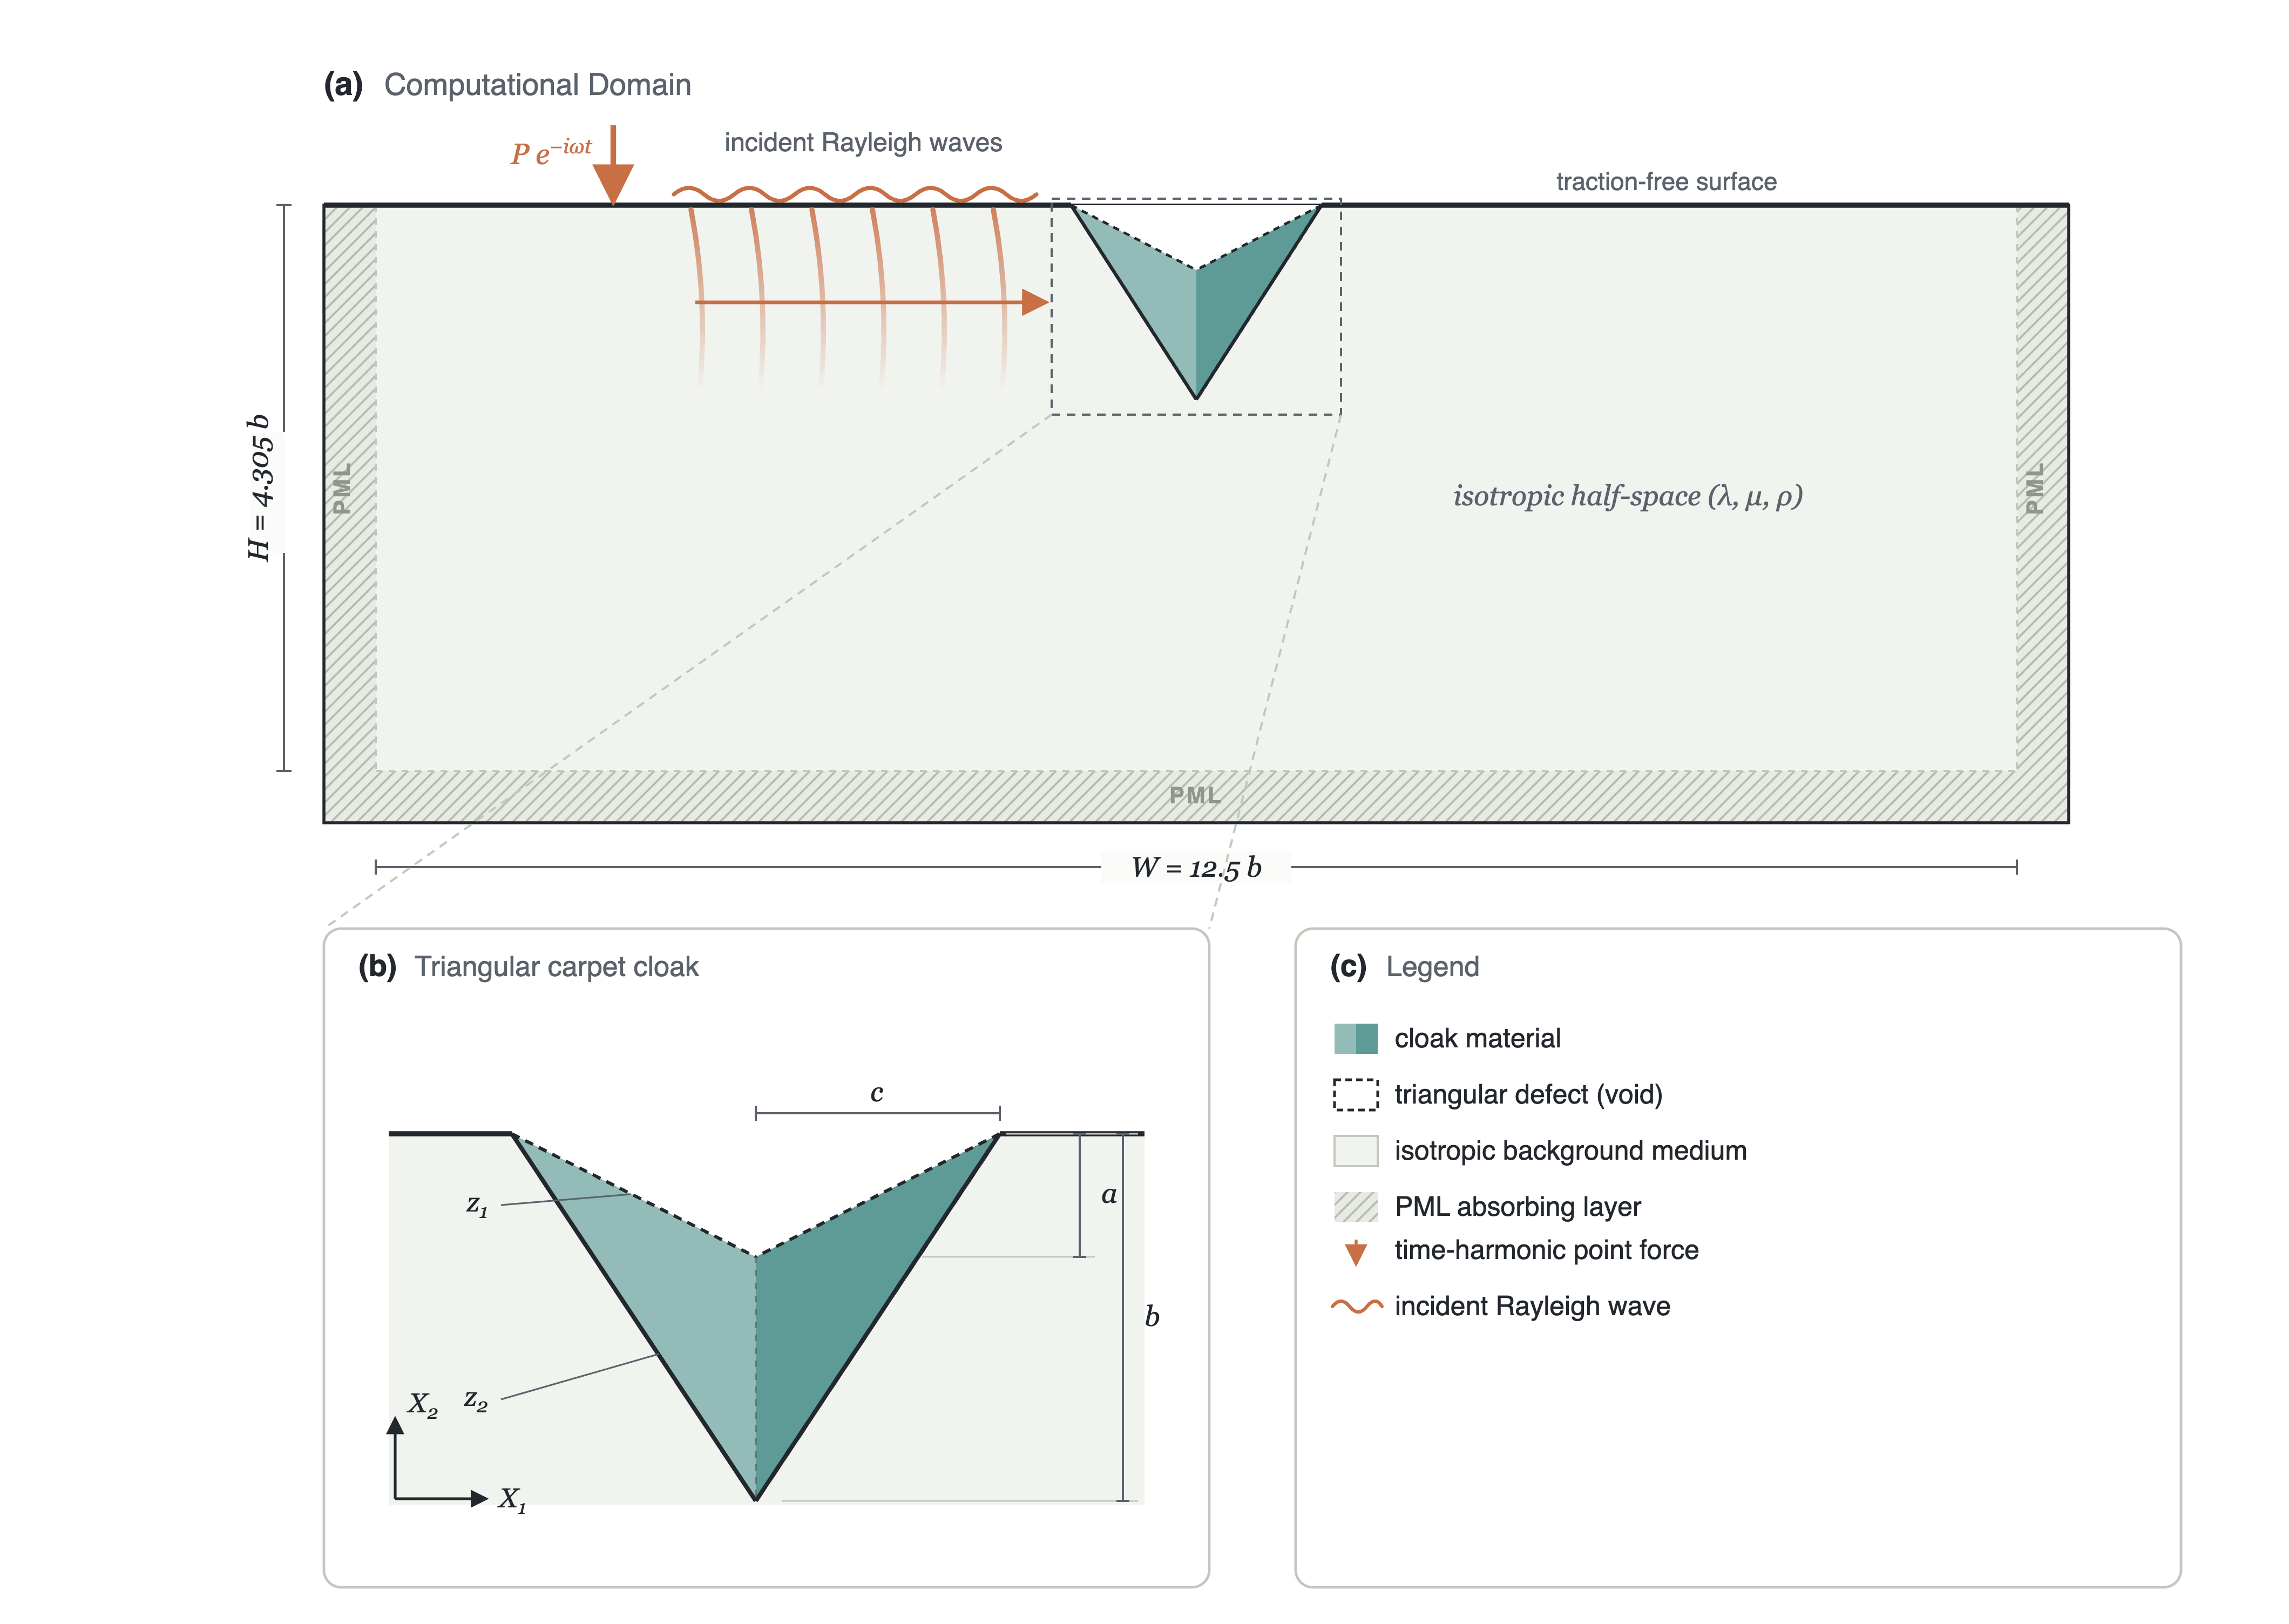
\includegraphics[width=\linewidth]{figures/problem-setup.png}
  \caption{Problem configuration. \textbf{(a)}~Computational domain:
  an isotropic elastic half-space $(\lambda,\mu,\rho)$ of width
  $W=12.5\,b$ is truncated by PML absorbing layers on the lateral and
  bottom boundaries; the top surface is traction-free. A time-harmonic
  vertical point force (red arrow) applied upstream generates Rayleigh
  waves (orange wavefronts) that propagate towards the triangular cloak
  (teal). \textbf{(b)}~Cloak geometry: the surface notch (void) has
  depth $a$ and half-width $c$; the outer cloak boundary sits at depth
  $b=3a$. Dashed lines mark the inner and outer triangle boundaries
  $z_1(X_1)$ and $z_2(X_1)$; the two mirror phases of the cloak are
  shaded in teal.}
  \label{fig:setup}
\end{figure}

\subsection{Governing equations}\label{subsec:governing}

We consider a homogeneous isotropic half-space with material properties
$(\lambda,\mu,\rho)$, where $\lambda$ and $\mu$ are the Lam\'e
coefficients and $\rho$ the mass density, and spatial coordinates
$\mbf{X}=(X_1,X_2)$ for the reference domain, with the free surface on
$X_2=0$. For in-plane surface waves, i.e.\ Rayleigh waves, propagating
along the horizontal $X_1$ direction, the governing Navier
elastodynamic equation the following form
\be\label{eq:navier_ref}
  \nabla_{\!X}\cdot\bigl(\mbf{C}:\nabla_{\!X}\mbf{U}\bigr)
  = \rho\,\mbf{U}_{tt},
\ee
where $\mbf{C}$ is the isotropic fourth-order elasticity tensor,
$\mbf{U}=(U_1,U_2)$ is the displacement, and $\mbf{U}_{tt}$ denotes its
second time derivative. Under the assumption of plane-strain
elasticity, the elastic tensor can be written in Voigt notation
$\{1,2,6\}=\{11,22,12\}$ as
\be\label{eq:Ciso}
  C_{IJ} =
  \begin{bmatrix}
    \lambda{+}2\mu & \lambda & 0 \\
    \lambda & \lambda{+}2\mu & 0 \\
    0 & 0 & \mu
  \end{bmatrix},
  \qquad I,J = 1,2,6.
\ee

We apply a pointwise invertible transformation $\Xi$ that maps the
reference configuration (virtual domain) $\mbf{X}\in\Psi$ to the
deformed region (physical domain) $\mbf{x}=\Xi(\mbf{X})\in\psi$ and the
remaining domain to itself. Given $\mbf{x}=(x_1,x_2)$ the coordinates
of the physical domain, the transformation gradient and its determinant
are
\be\label{eq:Fgrad}
  \mbf{F} = \nabla_{\!X}\,\mbf{x}
  =
  \begin{pmatrix}
    \dfrac{\partial x_1}{\partial X_1} & \dfrac{\partial x_1}{\partial X_2} \\[2mm]
    \dfrac{\partial x_2}{\partial X_1} & \dfrac{\partial x_2}{\partial X_2}
  \end{pmatrix},
  \qquad
  J = \det(\mbf{F}).
\ee
Equation~\eqref{eq:navier_ref} is not form-invariant under an arbitrary
transformation $\Xi$~\citep{milton2006}: the transformed material class
depends on the gauge $\mbf{U}(\Xi(\mbf{X}))=\mbf{A}\,\mbf{u}(\mbf{x})$
linking the virtual and physical displacements, with $\mbf{A}$ a
non-singular matrix. The choice $\mbf{A}=\mbf{F}$ leads to the Willis
setting, which guarantees a symmetric stress tensor but requires two
additional third-order coupling tensors and a tensorial mass
density~\citep{milton2006,norris2011,willis1981}, physically replicable
only within narrow frequency bands by resonant microstructures. For
this reason we adopt the Cosserat setting $\mbf{A}=\mbf{I}$, following
\citet{norris2011} and \citet{brun2009}, for which the governing
equation in the physical domain retains the Navier form
\be\label{eq:navier}
  \nabla_{\!x}\cdot\bigl(\mbf{c}^{\mathrm{eff}}:\nabla_{\!x}\mbf{u}\bigr)
  = \rho^{\mathrm{eff}}\,\mbf{u}_{tt},
\ee
with the transformed mechanical parameters given by the
Brun--Guenneau--Movchan (BGM) transformation relations
\be\label{eq:pushforward}
  c^{\mathrm{eff}}_{ijkl} = J^{-1}\,C_{IjKl}\,F_{iI}\,F_{kK},
  \qquad
  \rho^{\mathrm{eff}} = \rho\,J^{-1}.
\ee
The transformed tensor preserves the major symmetries
($c^{\mathrm{eff}}_{ijkl}=c^{\mathrm{eff}}_{klij}$) but not the minor
ones,
\be\label{eq:broken_minor}
  c^{\mathrm{eff}}_{ijkl}
  \neq c^{\mathrm{eff}}_{jikl}
  \neq c^{\mathrm{eff}}_{ijlk}
  \neq c^{\mathrm{eff}}_{jilk},
\ee
except for special cases such as conformal transformations. The medium
is nonetheless described by a single fourth-order, non-symmetric and,
eventually, inhomogeneous elastic tensor with scalar density: the
stress $\sigma_{ij}=c^{\mathrm{eff}}_{ijkl}\,\partial u_k/\partial x_l$
acts on the \emph{full} displacement gradient -- not the symmetric
strain -- and is itself non-symmetric (polar medium). All computations
below are carried out in the frequency domain with the time-harmonic
convention
$\mbf{u}(\mbf{x},t)=\operatorname{Re}\bigl[\mbf{u}(\mbf{x})\,e^{-\mathrm{i}\omega t}\bigr]$,
which replaces $\mbf{u}_{tt}$ by $-\omega^2\mbf{u}$.

\subsection{Transformation elasticity for the triangular carpet cloak}

The cloak follows the pinched-carpet construction
of \citet{chatzopoulos2023}. With the free surface on $X_2=0$ and the
cloak centred at $X_1=0$, the inner (defect) and outer cloak boundaries
are the triangles
\be\label{eq:triangles}
  z_1(X_1) = \frac{a}{c}\,|X_1| - a,
  \qquad
  z_2(X_1) = \frac{b}{c}\,|X_1| - b,
\ee
where $a$ is the defect depth, $b$ the cloak depth, and $c$ the surface
half-width. The shear map
\be\label{eq:shearmap}
  x_1 = X_1,
  \qquad
  x_2 = \frac{z_2(X_1)-z_1(X_1)}{z_2(X_1)}\,X_2 + z_1(X_1)
\ee
compresses the triangular region above $z_2$ onto the cloak region
between $z_1$ and $z_2$, opening the notch. Its gradient is piecewise
constant,
\be\label{eq:Ftensor}
  \mbf{F} =
  \begin{bmatrix} 1 & 0 \\ F_{21} & F_{22} \end{bmatrix},
  \qquad
  F_{21} = \operatorname{sign}(X_1)\,\frac{a}{c},
  \qquad
  F_{22} = \frac{b-a}{b} = J.
\ee
For an isotropic background $(\lambda,\mu)$ the BGM
push-forward~\eqref{eq:pushforward} then yields, in augmented Voigt
ordering $[\sigma_{11},\sigma_{22},\sigma_{12},\sigma_{21}]$, the
effective stiffness
\be\label{eq:Ceff}
  \mbf{c}_{\mathrm{eff}}
  =
  \begin{bmatrix}
    \dfrac{2\mu{+}\lambda}{F_{22}} & \lambda & 0 &
      \dfrac{F_{21}}{F_{22}}(2\mu{+}\lambda) \\[2mm]
    \lambda & \dfrac{F_{21}^2\mu + F_{22}^2(2\mu{+}\lambda)}{F_{22}} &
      \dfrac{F_{21}}{F_{22}}\,\mu & F_{21}(\lambda{+}\mu) \\[2mm]
    0 & \dfrac{F_{21}}{F_{22}}\,\mu & \dfrac{\mu}{F_{22}} & \mu \\[2mm]
    \dfrac{F_{21}}{F_{22}}(2\mu{+}\lambda) & F_{21}(\lambda{+}\mu) &
      \mu & \dfrac{F_{21}^2(2\mu{+}\lambda) + F_{22}^2\mu}{F_{22}}
  \end{bmatrix},
\ee
together with the constant effective density
\be\label{eq:rhoeff}
  \rho^{\mathrm{eff}} = \frac{\rho}{J} = \frac{b}{b-a}\,\rho.
\ee
Unlike radial blow-up cloaks, whose tensors are singular at the inner
boundary, the triangular tensor is non-singular and uniform within each
half of the cloak (the shear $F_{21}$ changes sign across the
centreline $X_1=0$), so the ideal cloak consists of just two
mirror-image material phases. The price is that \emph{three} minor
symmetry pairs are broken independently
($c_{11,12}\neq c_{11,21}$, $c_{22,12}\neq c_{22,21}$,
$c_{12,12}\neq c_{21,21}$), and these are the entries that
symmetrisation strategies average away by hand.

\subsection{Realisable Cauchy parameterisation}\label{subsec:flat4}

Throughout this paper the designed cloak is parameterised by four free
orthotropic Cauchy moduli $(C_{11},C_{12},C_{22},C_{66})$ (4CM) and a
scalar density, obtained by direct numerical search through the
differentiable FEM. This class is dictated by the microstructures that
must ultimately realise the cloak (Sec.~\ref{sec:micro}): square
two-phase unit cells invariant under the point group $D_2$, whose two
edge-aligned mirror axes fix the form of the homogenised stiffness.
Writing the plane-strain law in Voigt notation $\{1,2,6\}=\{11,22,12\}$,
a general symmetric Cauchy tensor has six independent constants,
\be\label{eq:cauchy_general}
  \begin{bmatrix}\sigma_{11}\\ \sigma_{22}\\ \sigma_{12}\end{bmatrix}
  =
  \begin{bmatrix}
    C_{11} & C_{12} & C_{16}\\
    C_{12} & C_{22} & C_{26}\\
    C_{16} & C_{26} & C_{66}
  \end{bmatrix}
  \begin{bmatrix}\varepsilon_{11}\\ \varepsilon_{22}\\ 2\varepsilon_{12}\end{bmatrix}.
\ee
The edge mirror $(x_1,x_2)\mapsto(x_1,-x_2)$ reverses the shear strain,
so requiring invariance $\mbf{C}=\mbf{T}\mbf{C}\mbf{T}$ with
$\mbf{T}=\operatorname{diag}(1,1,-1)$ forces $C_{16}=C_{26}=0$ and
reduces the stiffness to the block-diagonal orthotropic form
\be\label{eq:4cm}
  \mbf{C}_{\mathrm{4CM}}
  =
  \begin{bmatrix}
    C_{11} & C_{12} & 0\\
    C_{12} & C_{22} & 0\\
    0 & 0 & C_{66}
  \end{bmatrix},
\ee
whose four moduli are exactly the per-cell design variables. 

\subsection{Cell discretisation}

We discretise the cloak region into a regular Cartesian grid of
$n_x\times n_y$ square cells (Fig.~\ref{fig:cartesian_cells}). Cells
whose centre lies between the inner and outer triangles
\eqref{eq:triangles} are assigned a piecewise-constant effective
stiffness and the density~\eqref{eq:rhoeff}. Because the triangular
transformation is affine in Cartesian coordinates, the
tensor~\eqref{eq:Ceff} is passed to the FEM solver without any rotation
to a local frame. The ideal cloak tensor~\eqref{eq:Ceff} is the full $4\times4$
augmented-Voigt polar tensor with ten independent components. Because
real materials are Cauchy (minor-symmetric), the per-cell design variable
is four free orthotropic Cauchy moduli $(C_{11},C_{12},C_{22},C_{66})$
and a scalar density, which are searched numerically by the differentiable
optimiser. A systematic investigation of grid resolution established
$14\times10$ as the optimal discretisation, balancing approximation
fidelity against per-iteration computational cost; this resolution is
used in all single-frequency experiments reported below.

\begin{figure}[htbp]
  \centering
  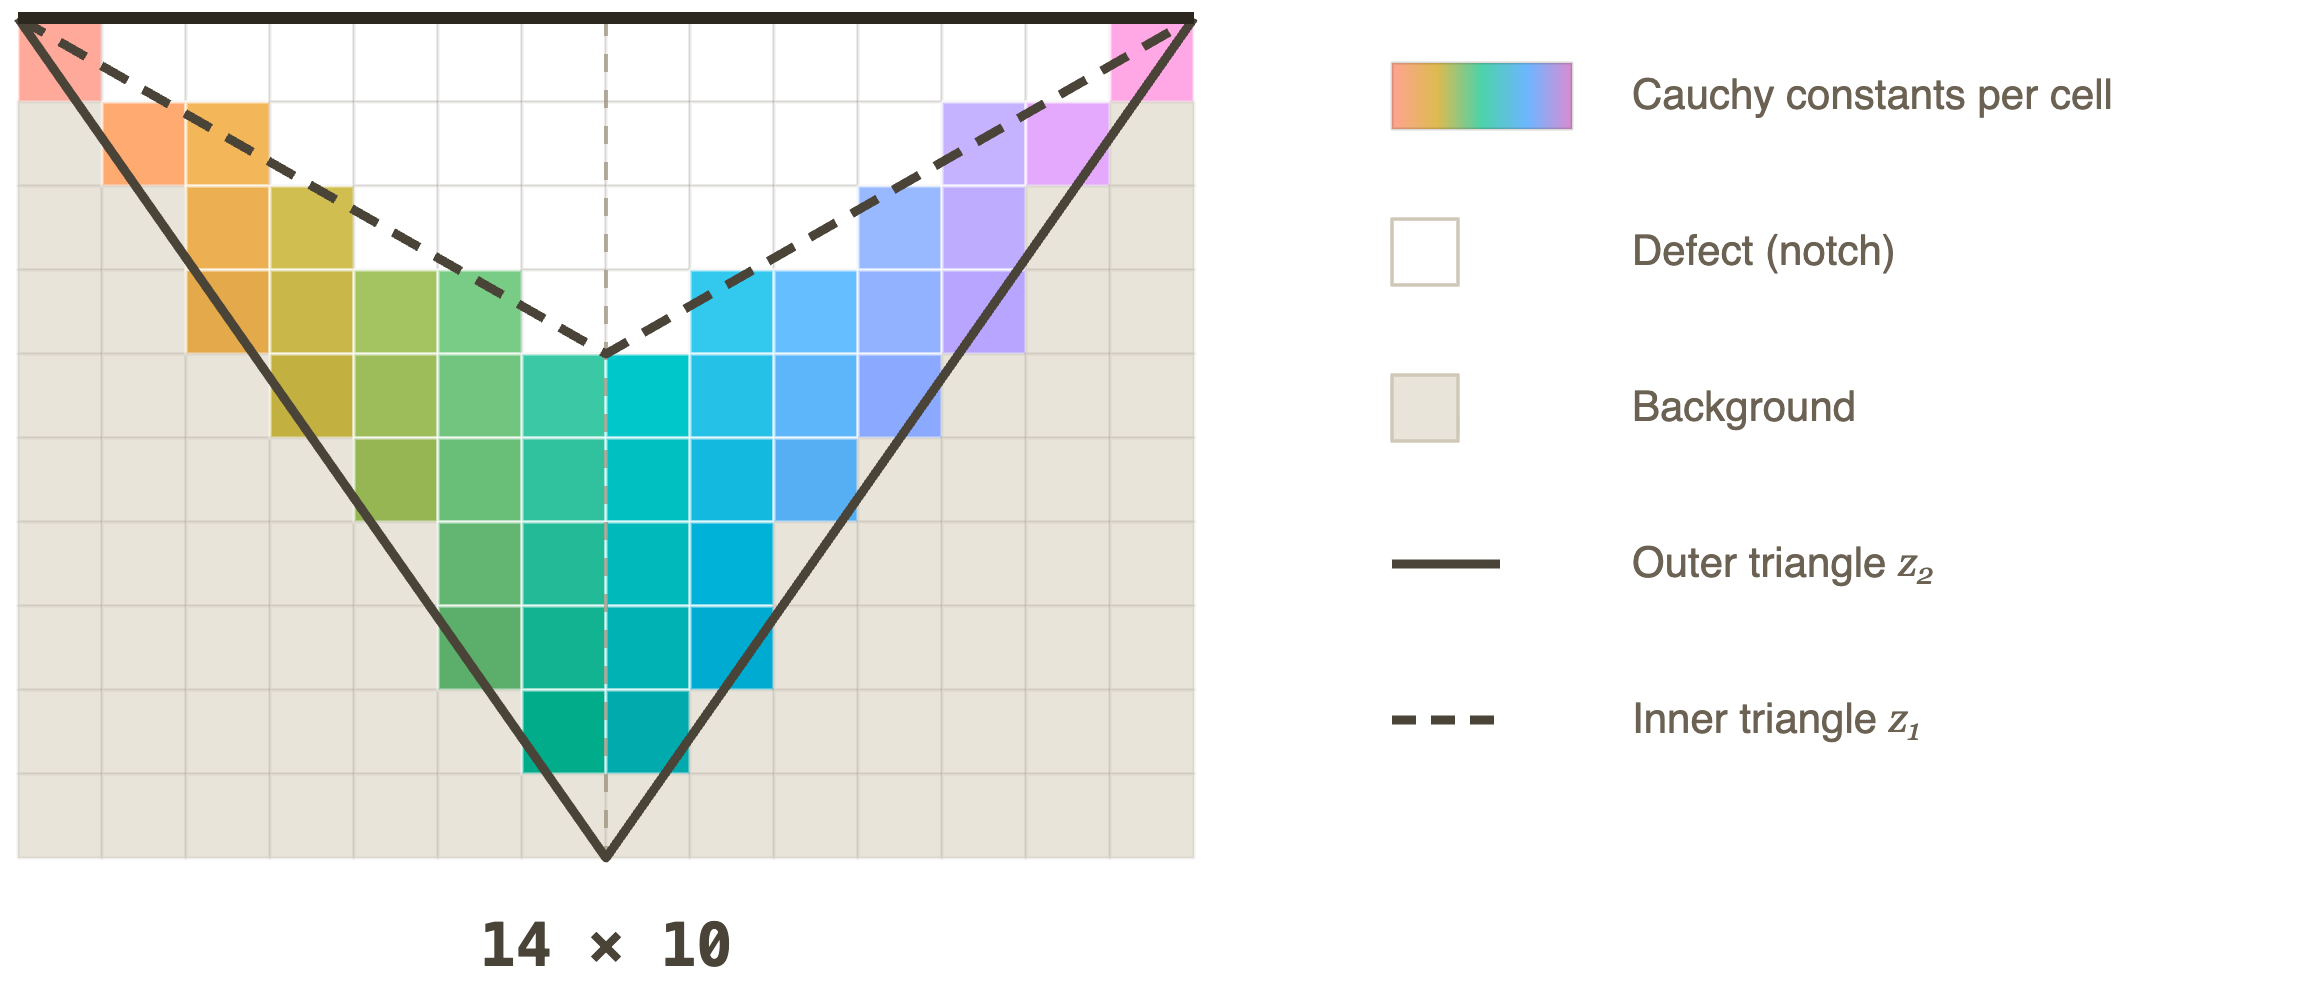
\includegraphics[width=0.75\linewidth]{figures/triangular-cell-decomposition.png}
  \caption{Cartesian cell decomposition of the triangular cloak at the
  $14\times10$ resolution used in all single-frequency experiments.
  Coloured cells carry per-cell Cauchy constants
  $(C_{11},C_{12},C_{22},C_{66},\rho)$; white cells lie inside the
  defect (void notch); grey cells are background. The solid line is the
  outer cloak boundary $z_2$ and the dashed line is the inner
  boundary $z_1$.}
  \label{fig:cartesian_cells}
\end{figure}

\subsection{Simulation domain and FEM solver}\label{subsec:domain}

We consider a rectangular computational domain of width $W=12.5\,b$ and
depth $H=4.305\,b$, truncating the half-space. The top boundary is
traction-free; PML absorbing layers terminate the two lateral
boundaries and the bottom. A triangular surface notch of depth
$a=0.0774\,H$ and half-width $c=0.1545\,H$ is centred on the free
surface, coated by a cloak of depth $b=3a$. The background medium is
isotropic with $\rho=1600\,\text{kg}/\text{m}^3$, shear speed
$c_s=300\,\text{m/s}$, and $c_p=\sqrt{3}\,c_s$
($\nu=1/4$, $\lambda=\mu=144\,\text{MPa}$, plane strain). The
excitation is a time-harmonic vertical point force applied on the free
surface upstream of the cloak, generating Rayleigh waves that propagate
along the surface towards the defect. Frequencies are reported in the
dimensionless form $f^\star = f\,b/c_R$, where $c_R\approx0.92\,c_s$ is
the Rayleigh wave speed of the background: at $f^\star=1$ the Rayleigh
wavelength equals the cloak depth $b$. The nominal design frequency is
$f^\star=2$.

The frequency-domain elastodynamic equations are solved with
complex-valued degrees of freedom and Rayleigh-damping PML through a
JAX-FEM finite-element solver~\citep{xu2020jaxfem} on a triangular mesh
with distance-based refinement near the cloak boundaries
($\sim\!246{,}000$ elements, $\sim\!124{,}000$ nodes). The entire
pipeline from cell material parameters through assembly and sparse
solve to the cloaking loss is differentiable via implicit adjoint
differentiation through the linear FEM solve, enabling gradient-based
optimisation of the per-cell stiffness and density.

\subsection{Cloaking metrics}

We use three relative $L^2$ metrics. The \emph{right-boundary
distortion}
\be\label{eq:distortion}
  \mathcal{D}_{\mathrm{r}}
  = 100\,\frac{\|\mbf{u}_{\mathrm{cloak}} - \mbf{u}_{\mathrm{ref}}\|_{L^2(\partial\Omega_{\mathrm{right}})}}
              {\|\mbf{u}_{\mathrm{ref}}\|_{L^2(\partial\Omega_{\mathrm{right}})}}\,,
\ee
measures the transmission-side mismatch with respect to the defect-free
reference. The \emph{outside-cloak distortion}
$\mathcal{D}_{\mathrm{out}}$ replaces the boundary integral by an
integral over $\Omega_{\mathrm{phys}}\setminus\overline{\Omega}_{\mathrm{cloak}}$ and
captures the global wavefield perturbation; it is closely related to
the objective used by \citet{wang2022}. In broadband sections we also
report the dimensionless cloak ratio
$\langle|\mbf{u}|\rangle/\langle|\mbf{u}_{\mathrm{ref}}|\rangle$ over
the free surface beyond the cloak footprint, following
\citet{chatzopoulos2023}; this is the cloaking objective used in the
microstructure-constrained pipeline.

\begin{figure}[htbp]
  \centering
  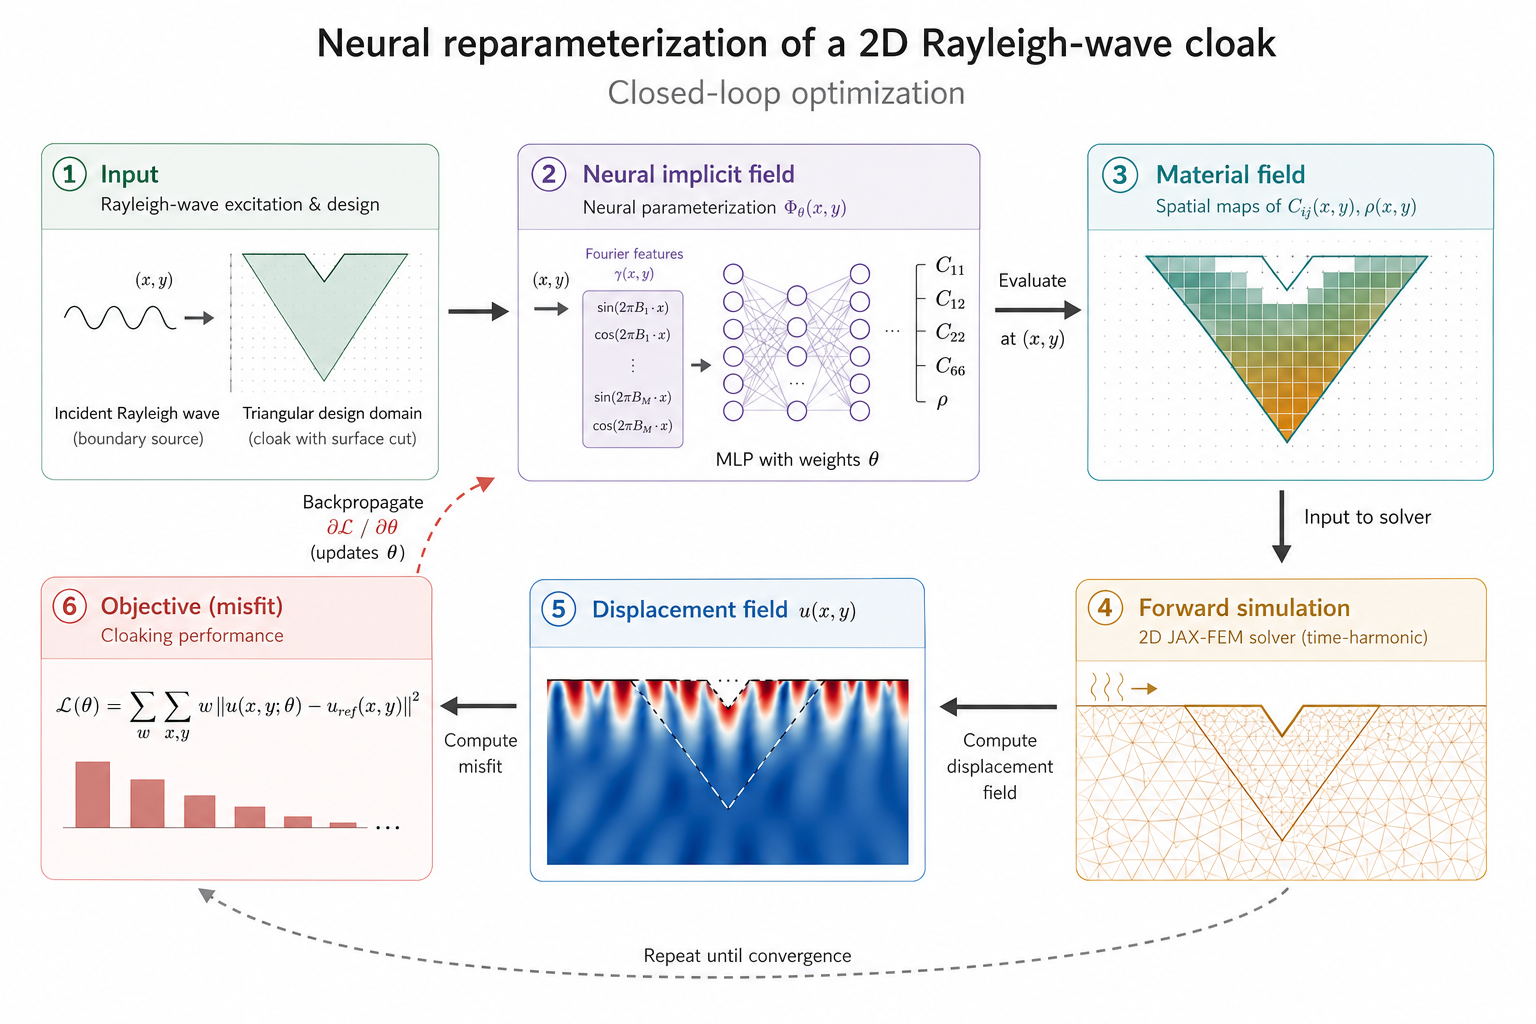
\includegraphics[width=0.95\linewidth]{figures/ml-pipeline.png}
  \caption{Neural-field design pipeline. Cell-centre coordinates are
  mapped through a Fourier positional encoding into a four-layer MLP
  that predicts the four free Cauchy moduli $(C_{11},C_{12},C_{22},C_{66})$
  and the density. The piecewise-constant material assignment is expanded to
  the FEM quadrature points and the cloaking objective is differentiated
  back through the implicit JAX-FEM adjoint into the network weights.}
  \label{fig:nf-arch}
\end{figure}

%% =============================================================
\section{Neural-field design pipeline}\label{sec:method}
%% =============================================================

\subsection{Coordinate-conditioned material network}

We reparameterise the cloak material field through a coordinate-based
multilayer perceptron (MLP)
\be\label{eq:neural_field}
  \Phi_\theta\colon(x,y)\;\mapsto\;(\mbf{C}_{\mathrm{4CM}}(x,y),\,\rho(x,y)),
\ee
where $\theta$ denotes the network weights,
$\mbf{C}_{\mathrm{4CM}}\in\mathbb{R}^{4}$ contains the four free Cauchy
moduli $(C_{11},C_{12},C_{22},C_{66})$ — the design variables directly
searched by the optimiser — and $\rho$ is a positive scalar density. The network
is evaluated at each cloak-cell centre to produce the piecewise-constant
material assignment that is then expanded to the FEM quadrature points.
A four-layer MLP with 256 hidden units ($\sim\!200{,}000$ weights) is
used in all experiments; we adopt $\tanh$ activations and the Fourier
positional encoding of \citet{tancik2020fourier} so that the network
can represent sharp material transitions near the cloak boundaries.

Figure~\ref{fig:nf-arch} shows the architecture and the data flow
through the differentiable FEM. Gradients
$\partial\mathcal{L}/\partial\theta$ are obtained by backpropagating
through the JAX-FEM adjoint solve and into the network.

\subsection{Transformation-elasticity prior}

The network does not learn the cloak from scratch. The four Cauchy moduli
per cell are initialised at a starting point $\mbf{C}_{\mathrm{4CM}}^{(0)}$
and then freely optimised. We tried two choices for this starting point -- the 
arithmetic-mean symmetrisation of the ideal tensor~\eqref{eq:Ceff} and the mean of the
microstructure dataset (Sec.~\ref{sec:micro}) -- and found no statistically
significant difference in the converged results, indicating that the design
is driven by the cloaking objective rather than by the initialisation.
Concretely, the last layer is scaled near zero
($\mbf{W}\leftarrow 0.01\,\mbf{W},\;\mbf{b}\leftarrow\mbf{0}$) and the
network output is applied as a \emph{multiplicative residual} with default
output scale $\epsilon=0.1$:
\begin{subequations}\label{eq:neural_relative}
\begin{align}
  \mbf{C}_{\mathrm{4CM}}(x,y)
    &= \mbf{C}_{\mathrm{4CM}}^{(0)}(x,y)\odot
       \bigl(1+\epsilon\,\Phi_\theta^{(C)}(x,y)\bigr),
       \label{eq:neural_relative_C}\\
  \rho(x,y)
    &= \rho^{(0)}(x,y)\bigl(1+\epsilon\,\Phi_\theta^{(\rho)}(x,y)\bigr).
       \label{eq:neural_relative_rho}
\end{align}
\end{subequations} The multiplicative form makes
the relative perturbation spatially uniform regardless of the orders of
magnitude separating the stiffness and density entries within each
cloak phase. An additive variant is also implemented but produces more
poorly conditioned gradients in practice.

\subsection{Physical admissibility of the material output}\label{sec:constrained}

The multiplicative residual~\eqref{eq:neural_relative} places no bound on
the sign or the anisotropy of the moduli: an unconstrained MLP can drive
a stiffness negative, break the positive-definiteness of the Cauchy
tensor, or reach an anisotropy ratio no real microstructure can realise.
Rather than police these violations with penalty terms after the fact, we
build them into the decoding, so that \emph{every} network output --- at
initialisation, along the optimisation path, and at convergence --- is a
physically admissible material by construction. The optimiser therefore
searches only over the manifold of valid tensors and never has to be
projected back onto it.

The network still emits four unbounded raw channels
$\mbf{r}=(r_{11},r_{22},r_{66},r_{12})=\Phi_\theta^{(C)}(x,y)$ per cloak
cell, but these are mapped to the moduli through three guarantees.

\emph{(i) Positive diagonal and shear.} The three positive-definite
entries are set by a log-space (hence strictly positive) multiplicative
residual,
\be\label{eq:constr_diag}
  C_{ii} = C_{ii}^{(0)}\,\exp(\epsilon\,r_{ii}),
  \qquad ii\in\{11,22,66\},
\ee
which keeps them positive for any real $r_{ii}$ and recovers
$C_{ii}^{(0)}$ at $\mbf{r}=\mbf 0$.

\emph{(ii) Bounded anisotropy.} To exclude ratios beyond what the
microstructure can attain, the diagonal ratio $C_{11}/C_{22}$ is confined
to $[1/R,\,R]$ while its geometric mean $\sqrt{C_{11}C_{22}}$ is held
fixed. Writing $g=\tfrac12\log(C_{11}/C_{22})$, a $\tanh$ squash on the
half-log ratio,
\be\label{eq:constr_aniso}
  g_b = \tfrac12\log R\,\tanh\!\Bigl(\tfrac{g}{\tfrac12\log R}\Bigr),
  \qquad
  C_{11},C_{22}=\sqrt{C_{11}C_{22}}\;e^{\pm g_b},
\ee
bounds the ratio smoothly to $[1/R,R]$ with $R$ the anisotropy cap (we
use $R=30$, chosen above the $99$th percentile of the microstructure
dataset with margin).

\emph{(iii) Positive-definite coupling.} The off-diagonal $C_{12}$ is
written through a correlation coefficient $\rho_c\in(-\kappa,\kappa)$
rather than directly,
\be\label{eq:constr_c12}
  C_{12}=\rho_c\,\sqrt{C_{11}C_{22}},
  \qquad
  \rho_c=\kappa\,\tanh\!\bigl(r_{12}+\phi_0\bigr),
\ee
with $\kappa<1$ (we use $\kappa=0.99$). Because $|\rho_c|<\kappa<1$, the
orthotropic block stays strictly positive-definite,
$\det=C_{11}C_{22}(1-\rho_c^2)>0$, for any $r_{12}$, and $C_{12}$ is free
to change sign. The offset $\phi_0=\operatorname{arctanh}(\rho_c^{(0)}/\kappa)$
centres the map so that $\mbf{r}=\mbf 0$ again recovers the initial
coupling $C_{12}^{(0)}$. Non-cloak cells bypass the decoding and keep
their background values exactly.

Together, \eqref{eq:constr_diag}--\eqref{eq:constr_c12} turn the raw
network outputs into a smooth, everywhere-differentiable surjection onto
the set of positive-definite, bounded-anisotropy Cauchy tensors, so the
transformation-elasticity initialisation is recovered at $\mbf{r}=\mbf 0$
and every gradient step lands on an admissible design.

\subsection{Loss function}

The optimisation minimises a
\emph{magnitude-band integral}: the mean-squared relative error of the
displacement magnitude over a strip of depth $d=0.5\,b$ (half the cloak
depth) below the free surface, downstream of and excluding the
cloak/defect footprint,
\begin{subequations}\label{eq:opt_loss_cloak}
\begin{align}
  \mcl{L}_{\mathrm{cloak}}(\theta)
  &= \frac{1}{|\mcl{B}|}\int_{\mcl{B}}
      \left(\frac{|\mbf{u}_{\mathrm{cloak}}|}{|\mbf{u}_{\mathrm{ref}}|}-1\right)^{2}
      \,\mathrm{d}A, \label{eq:opt_loss_cloak_L}\\
  \mcl{B}&=\bigl\{(x,y)\in\Omega_{\mathrm{phys}}\setminus\overline{\Omega}_{\mathrm{cloak}}
     : y_{\mathrm{top}}-d\le y\le y_{\mathrm{top}},\ x>x_c\bigr\}.
     \label{eq:opt_loss_cloak_B}
\end{align}
\end{subequations}
where $\mbf{u}_{\mathrm{cloak}}$ and $\mbf{u}_{\mathrm{ref}}$ are the
cloaked and defect-free reference fields and $x_c$ is the downstream edge
of the cloak. Comparing magnitudes rather than the complex fields
themselves makes the objective phase-invariant, which is a
deliberate advantage here: a wave
that is diverted around the defect follows a slightly longer path and
arrives with a small phase lag relative to the flat-surface reference.
An explicit
neighbour-smoothness term used in raw-parameter
baselines~\citep{wang2022} is unnecessary here: the neural field is
spatially continuous by construction, and its smoothness is controlled
directly through the Fourier positional
encoding~\citep{tancik2020fourier}. The number and bandwidth of the
Fourier features set the spatial frequency content the network can
represent---low frequencies yield smooth, gently varying material fields,
whereas adding higher-frequency components lets the field resolve sharper
transitions near the cloak boundaries. 

%% =============================================================
\section{Single-frequency results}\label{sec:single_freq}
%% =============================================================

All single-frequency results are reported at the design frequency
$f^\star=2.0$ through the dimensionless \emph{cloak ratio}
\be\label{eq:cloak_ratio}
  \eta \;=\;
  \frac{\langle|\mbf{u}|\rangle}{\langle|\mbf{u}_{\mathrm{ref}}|\rangle}
\ee
of the mean surface-displacement magnitude on the free surface beyond the
cloak footprint to that of the defect-free reference (Sec.~\ref{sec:setup}),
so that $\eta\to1$ is perfect cloaking and $|1-\eta|$ measures the residual
distortion. We build up the design in three steps of increasing material
freedom: a single homogeneous realisable material
(Sec.~\ref{subsec:single_material}), a handful of independent materials
(Sec.~\ref{subsec:four_materials}), and finally a cell grid selected by a
convergence sweep (Secs.~\ref{subsec:grid_selection}--\ref{subsec:final14}).

\subsection{A single realisable material already beats symmetrisation}
\label{subsec:single_material}

We first ask how far a \emph{single} realisable material can go. Both cloak
phases are collapsed onto one orthotropic 4CM tile (a $1\times1$ cell filling
the whole cloak) and its four Cauchy moduli $(C_{11},C_{12},C_{22},C_{66})$
and density are searched by the differentiable FEM at $f^\star=2.0$. The
natural point of comparison is the closed-form arithmetic-mean symmetrisation
of \citet{chatzopoulos2023}: the ideal polar tensor~\eqref{eq:Ceff} made
minor-symmetric by averaging each broken pair, instantiated on the same mesh
and solved with the same FEM. Both are single homogeneous Cauchy materials,
so this is a like-for-like test of hand symmetrisation against direct search.

Table~\ref{tab:single_vs_sym} reports the outcome. The symmetrised tensor
recovers only $\eta=0.63$ and actually distorts the near field more than the
bare notch (the ideal-material minor-symmetry violation is large at
$f^\star=2$). A single searched orthotropic material instead reaches
$\eta=0.85$ --- a substantial jump towards the ideal continuous polar cloak
($\eta=0.999$) obtained from just one degree of material freedom per phase,
and clear evidence that direct search inside the Cauchy class outperforms
symmetrisation. It is, however, still far from perfect: one material cannot
reproduce the depth variation of the ideal tensor.
Figure~\ref{fig:single_vs_sym_sweep} confirms that the advantage is
concentrated around the design frequency, as expected for a single-frequency
optimisation.

\begin{table}[htbp]
\centering
\caption{Single-frequency cloak ratio $\eta$~\eqref{eq:cloak_ratio} at
$f^\star=2.0$ for a single homogeneous realisable material. A single
orthotropic 4CM tile found by direct search ($\eta=0.85$) markedly
outperforms the closed-form arithmetic-mean symmetrisation of
\citet{chatzopoulos2023} ($\eta=0.63$), but neither reaches the ideal
continuous polar cloak. Values from \texttt{output/A\_symmetrized} and
\texttt{output/A\_1x1flat4\_vs\_symmetrized}.}
\label{tab:single_vs_sym}
\begin{tabular*}{\textwidth}{@{\extracolsep{\fill}}lcc@{}}
\toprule
Configuration & $\eta$ & $|1-\eta|$ \\
\midrule
Uncoated notch (no cloak)                                   & $0.37$  & $0.63$ \\
Symmetrised ideal (Chatzopoulos, closed-form Cauchy)        & $0.634$ & $0.366$ \\
Single optimised material ($1\times1$, 4CM)                 & $0.850$ & $0.150$ \\
\midrule
Ideal continuous $\mbf{c}_{\mathrm{eff}}$ (polar, unrealisable) & $0.999$ & $0.001$ \\
\bottomrule
\end{tabular*}
\end{table}

\begin{figure}[htbp]
  \centering
  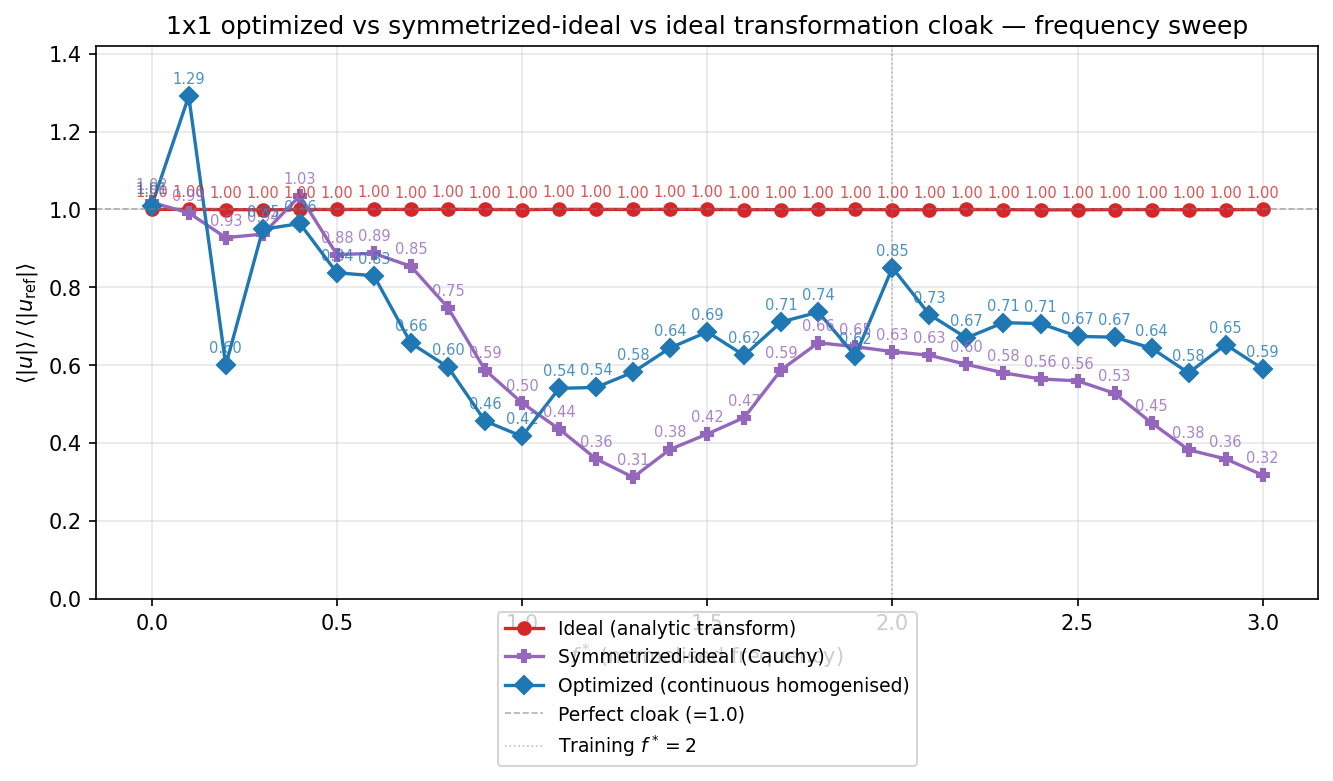
\includegraphics[width=0.9\linewidth]{figures/single_vs_symmetrized_sweep.png}
  \caption{Frequency sweep of the cloak ratio
  $\eta=\langle|\mbf{u}|\rangle/\langle|\mbf{u}_{\mathrm{ref}}|\rangle$ for the
  single-material designs: the ideal continuous transformation cloak
  (red, $\eta\approx1$ at every frequency), the closed-form symmetrised
  tensor of \citet{chatzopoulos2023} (purple), and the single optimised
  $1\times1$ material (blue). At the training frequency $f^\star=2$ the
  optimised material recovers $\eta=0.85$ against $0.63$ for symmetrisation.}
  \label{fig:single_vs_sym_sweep}
\end{figure}

\subsection{Four materials reach $95\%$ cloaking}\label{subsec:four_materials}

Giving each phase more freedom closes most of the remaining gap. Splitting
the cloak into a coarse $n_x\times n_y$ grid of independent orthotropic tiles
and optimising all of them jointly, we find that even a $2\times2$
decomposition --- just \emph{four} realisable materials --- lifts the cloak
ratio to $\eta=0.962$, i.e.\ within $4\%$ of a perfect cloak
(Table~\ref{tab:partition}). The improvement is markedly anisotropic:
subdividing in depth helps far more than in the propagation direction
($1\times2$ reaches $\eta=0.92$ whereas $2\times1$ actually drops to
$\eta=0.78$), reflecting that the ideal cloak material varies mainly with
depth through the shear map~\eqref{eq:shearmap}. Beyond four materials the
gain per added cell is small, motivating a more systematic grid study.

\begin{table}[htbp]
\centering
\caption{Single-frequency cloak ratio $\eta$ for small cell decompositions
of the cloak (each cell is one independent orthotropic 4CM material, all
optimised jointly at $f^\star=2.0$). Four materials ($2\times2$) already
reach $\eta=0.962$. Values from \texttt{output/A\_partition\_pushed}.}
\label{tab:partition}
\begin{tabular*}{\textwidth}{@{\extracolsep{\fill}}lccc@{}}
\toprule
Decomposition $n_x\times n_y$ & Materials & $\eta$ & $|1-\eta|$ \\
\midrule
$1\times1$          & 1 & $0.857$ & $0.143$ \\
$2\times1$          & 2 & $0.780$ & $0.220$ \\
$1\times2$          & 2 & $0.920$ & $0.080$ \\
$3\times1$          & 3 & $0.939$ & $0.061$ \\
$\mathbf{2\times2}$ & \textbf{4} & $\mathbf{0.962}$ & $\mathbf{0.038}$ \\
$3\times2$          & 6 & $0.964$ & $0.036$ \\
\bottomrule
\end{tabular*}
\end{table}

\subsection{Grid selection by a cell-convergence sweep}
\label{subsec:grid_selection}

To push towards perfect cloaking we refine the grid, but the resolution must
be chosen so that cloaking has \emph{converged} while the per-iteration cost
stays low. We therefore run a single-frequency cell sweep over seven
Cartesian grids from $5\times4$ to $32\times24$, optimising each to
convergence and recording the cloak ratio
(Table~\ref{tab:cell_sweep}, Fig.~\ref{fig:cell_sweep}).

A key point is that materials are assigned only to cells whose centre falls
between the inner and outer triangles~\eqref{eq:triangles}, so an
$n_x\times n_y$ grid uses far fewer than $n_x n_y$ materials: the triangular
cloak occupies only a fraction of its Cartesian bounding box. The
$14\times10$ grid nominally spans $140$ cells but places only
\textbf{46 cells inside the cloak region}; these $46$ are the actual design
variables, the remaining $94$ being background. (The figures in
parentheses in Fig.~\ref{fig:cell_sweep} are these in-cloak counts:
$5\times4\!\to\!7$, $8\times6\!\to\!16$, $10\times8\!\to\!28$,
$14\times10\!\to\!46$, and so on.)

The cloak ratio saturates on a plateau at $\eta\approx0.99$
($|1-\eta|\approx0.01$) by $14\times10$: the three finer grids
($20\times15$, $26\times20$, $32\times24$) give no further improvement --- and
even a marginal regression from FEM cost and optimisation noise --- while
their cell counts, and hence solve cost, grow several-fold. The $14\times10$
grid is the smallest decomposition sitting firmly on this converged
sub-$1\%$ plateau, and we adopt it for all subsequent single-frequency
work: it is stable (on the flat part of the curve), cheap (only $46$ active
materials), and fast to optimise.

\begin{table}[htbp]
\centering
\caption{Single-frequency cell-convergence sweep at $f^\star=2.0$. Each grid
is optimised to convergence; ``cloak cells'' is the number of cells whose
centre lies inside the triangular cloak and therefore carries design
variables (far fewer than $n_x n_y$). The cloak ratio plateaus at
$\eta\approx0.99$ by $14\times10$; finer grids do not improve it. Values from
\texttt{output/A\_cell\_sweep}.}
\label{tab:cell_sweep}
\begin{tabular*}{\textwidth}{@{\extracolsep{\fill}}lcccc@{}}
\toprule
Grid $n_x\times n_y$ & Total cells & Cloak cells & $\eta$ & $|1-\eta|$ \\
\midrule
$5\times4$            & 20  & 7   & $0.944$ & $0.056$ \\
$8\times6$            & 48  & 16  & $0.943$ & $0.057$ \\
$10\times8$           & 80  & 28  & $0.977$ & $0.023$ \\
$\mathbf{14\times10}$ & \textbf{140} & \textbf{46} & $\mathbf{0.990}$ & $\mathbf{0.010}$ \\
$20\times15$          & 300 & 100 & $0.990$ & $0.010$ \\
$26\times20$          & 520 & 176 & $0.988$ & $0.012$ \\
$32\times24$          & 768 & 256 & $0.988$ & $0.012$ \\
\bottomrule
\end{tabular*}
\end{table}

\begin{figure}[htbp]
  \centering
  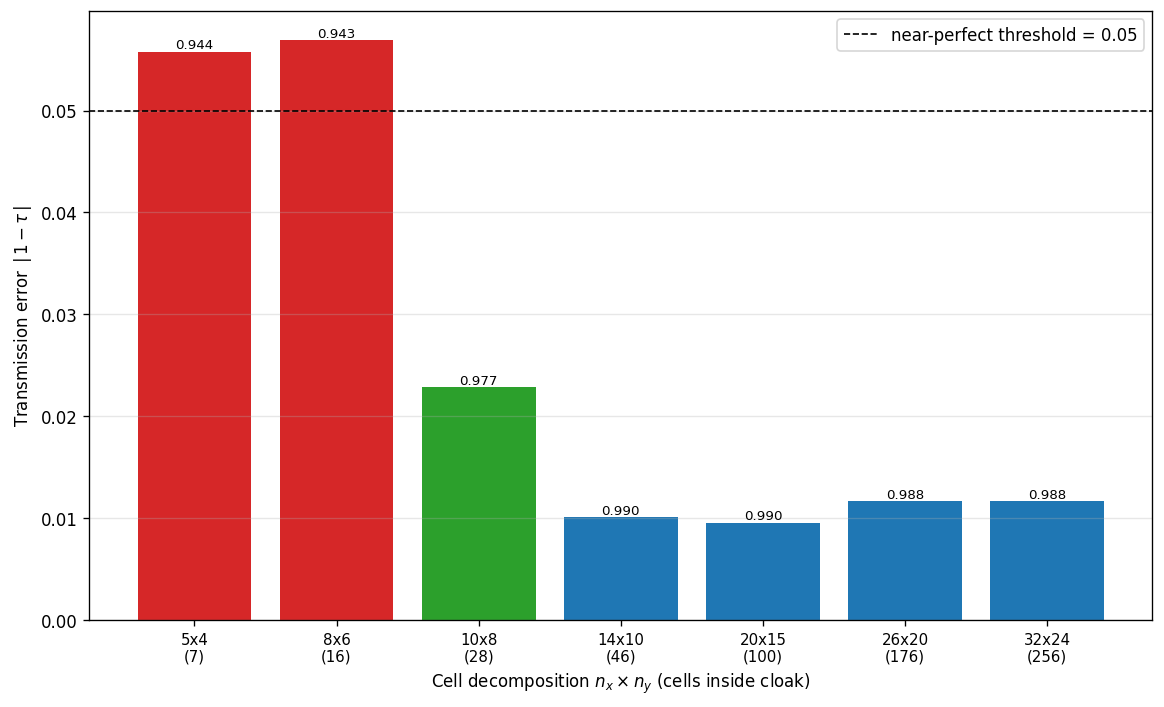
\includegraphics[width=0.8\linewidth]{figures/cell_sweep_histogram.png}
  \caption{Cloaking error $|1-\eta|$ versus cell decomposition in the
  single-frequency sweep; numbers in parentheses on the axis are the
  in-cloak cell counts. The error drops sharply up to $10\times8$
  ($28$ cloak cells) and then flattens: $14\times10$ ($46$ cloak cells) is
  the smallest grid on the converged sub-$1\%$ plateau, with finer grids
  giving no further improvement.}
  \label{fig:cell_sweep}
\end{figure}

\subsection{Near-perfect cloaking on the $14\times10$ grid}\label{subsec:final14}

The adopted $14\times10$ design ($46$ optimised in-cloak materials) reaches
$\eta=0.990$, effectively closing the gap to the ideal continuous cloak.
Figure~\ref{fig:single14_field} compares the real-displacement magnitude of
the optimised cloak against three references on the same mesh: the defect-free
reference, the uncloaked notch, and the ideal continuous polar
$\mbf{c}_{\mathrm{eff}}$. The uncloaked notch back-scatters the incident
Rayleigh wave and casts a clear shadow downstream; the optimised $14\times10$
cloak restores the surface wavefield to the reference, matching the ideal
continuous cloak panel while using only realisable orthotropic Cauchy
materials. The only visible residual is a slight phase shift of the optimised solution:
Figure~\ref{fig:single14_zoom} zooms into the cloak region and shows that,
whereas the ideal continuous cloak keeps its near-surface wavefronts
phase-aligned with the reference, the optimised $14\times10$ cloak carries them
$\approx0.18\lambda$ ($\approx65^\circ$) later. This lag is a direct and benign
consequence of the phase-invariant magnitude loss~\eqref{eq:opt_loss_cloak}:
the objective constrains only the amplitude envelope, leaving a constant phase
offset --- the small extra path of a wave routed around the notch ---
unpenalised.
Figure~\ref{fig:single14_material} shows the corresponding
optimised per-cell moduli $(C_{11},C_{22},C_{12},C_{66})$ and density over
the $46$ cloak cells.

\begin{figure}[htbp]
  \centering
  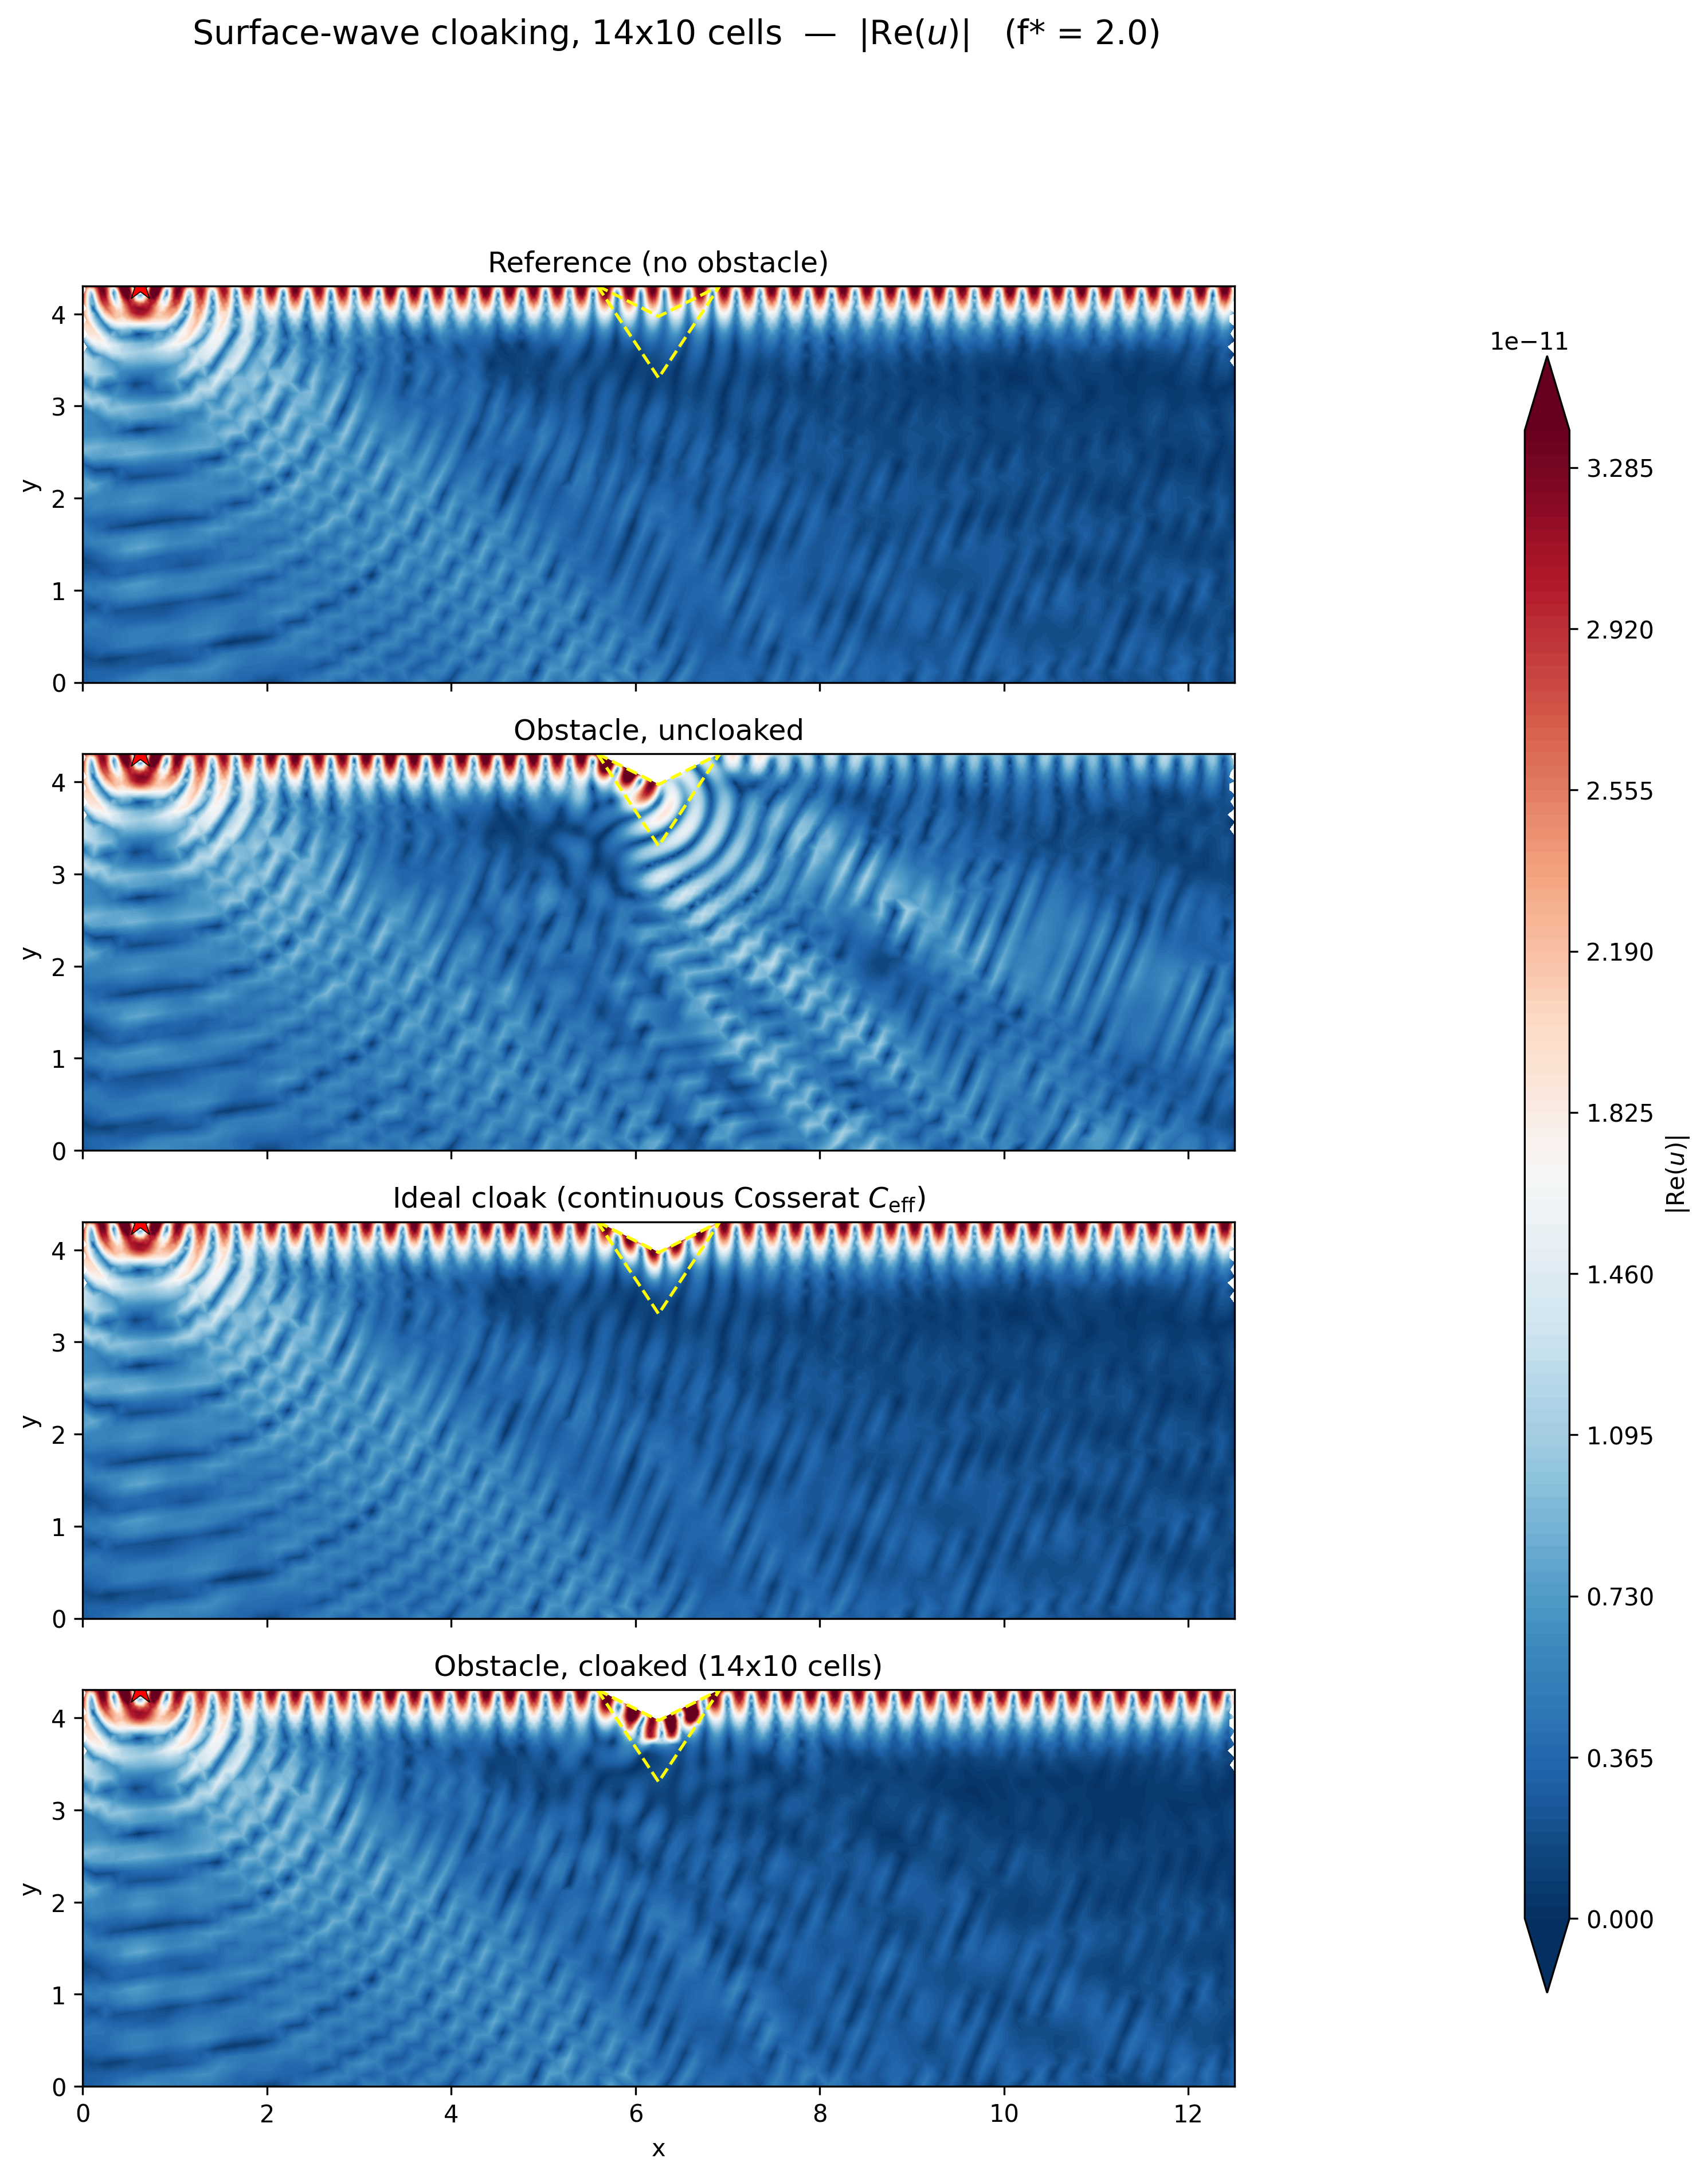
\includegraphics[width=0.82\linewidth]{figures/single_freq_14x10_re_mag.png}
  \caption{Real-displacement magnitude $|\!\operatorname{Re}\mbf{u}|$ at
  $f^\star=2.0$ (top to bottom): defect-free reference, uncloaked notch,
  ideal continuous polar cloak $\mbf{c}_{\mathrm{eff}}$, and the optimised
  $14\times10$-cell cloak ($46$ in-cloak materials, $\eta=0.990$). The
  optimised cloak reconstructs the reference wavefield on the transmission
  side and is visually indistinguishable from the ideal continuous cloak,
  with the downstream shadow of the uncloaked notch removed. Dashed lines
  mark the cloak/defect boundary.}
  \label{fig:single14_field}
\end{figure}

\begin{figure}[htbp]
  \centering
  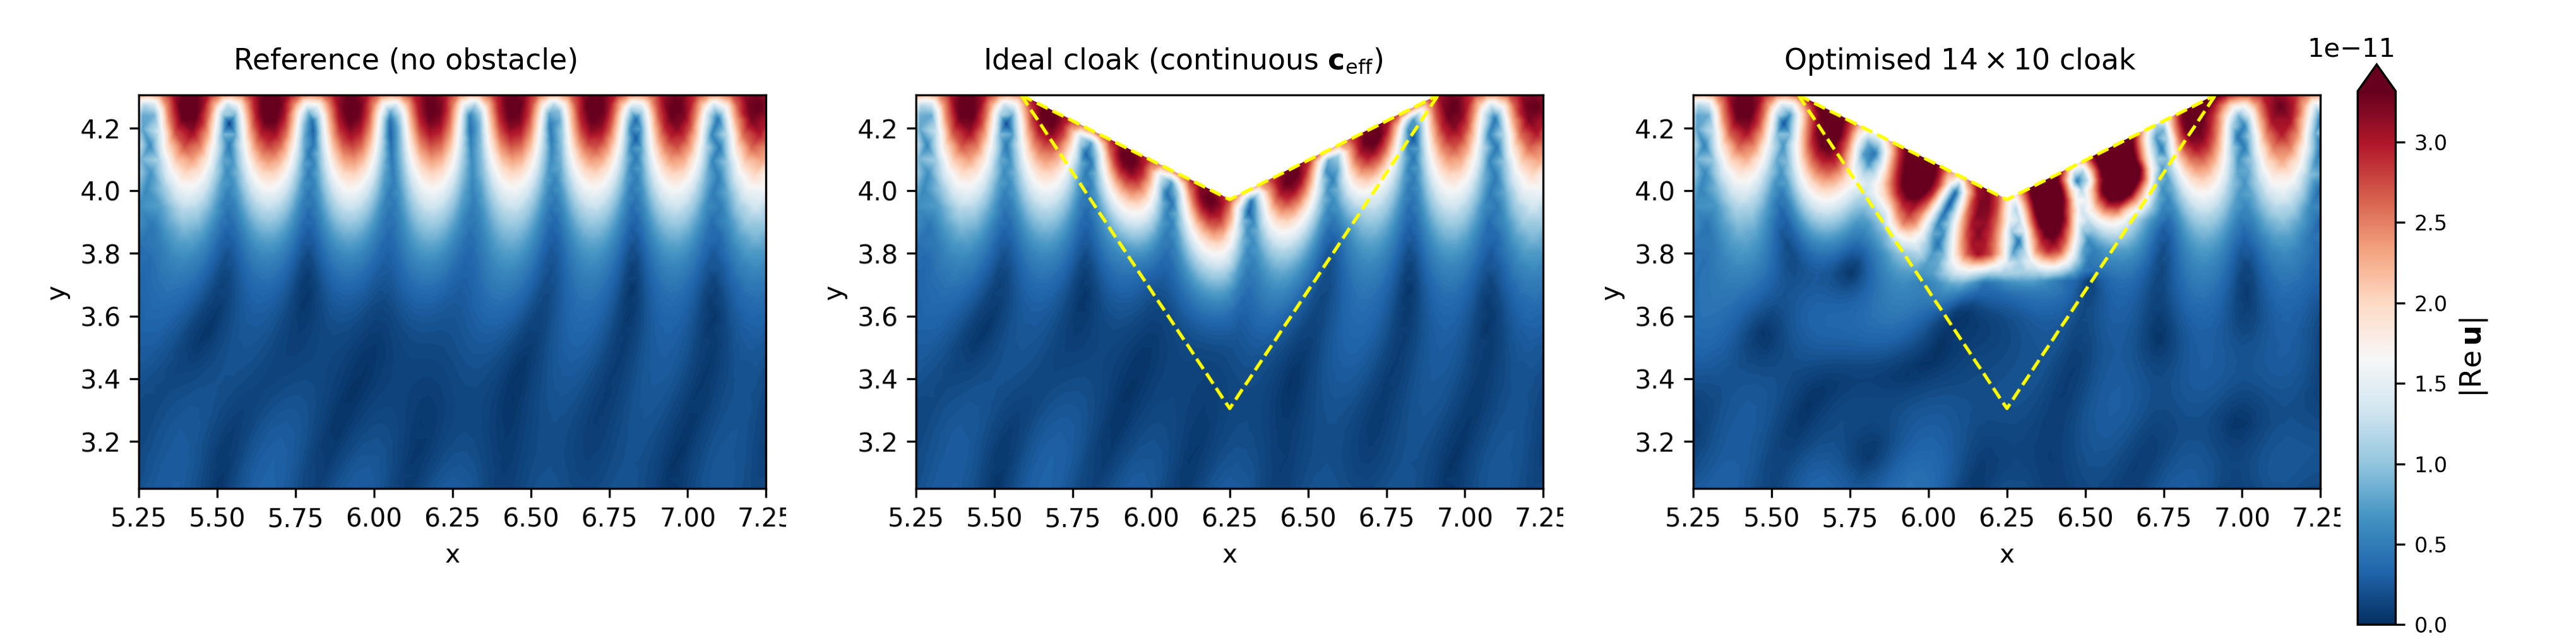
\includegraphics[width=\linewidth]{figures/single_freq_14x10_zoom_phase.png}
  \caption{Zoom on the cloak region ($|\!\operatorname{Re}\mbf{u}|$ at
  $f^\star=2.0$, shared colour scale): defect-free reference (left), ideal
  continuous polar cloak (centre), and optimised $14\times10$ cloak (right);
  dashed lines outline the inner (defect) and outer cloak boundaries. All three
  reproduce the same amplitude envelope, but the optimised cloak leaves its
  near-surface wavefronts slightly phase-shifted ($\approx0.18\lambda$,
  $\approx65^\circ$) relative to the reference and the ideal cloak --- a
  constant phase offset left unconstrained by the phase-invariant magnitude
  loss, not a cloaking error.}
  \label{fig:single14_zoom}
\end{figure}

\begin{figure}[htbp]
  \centering
  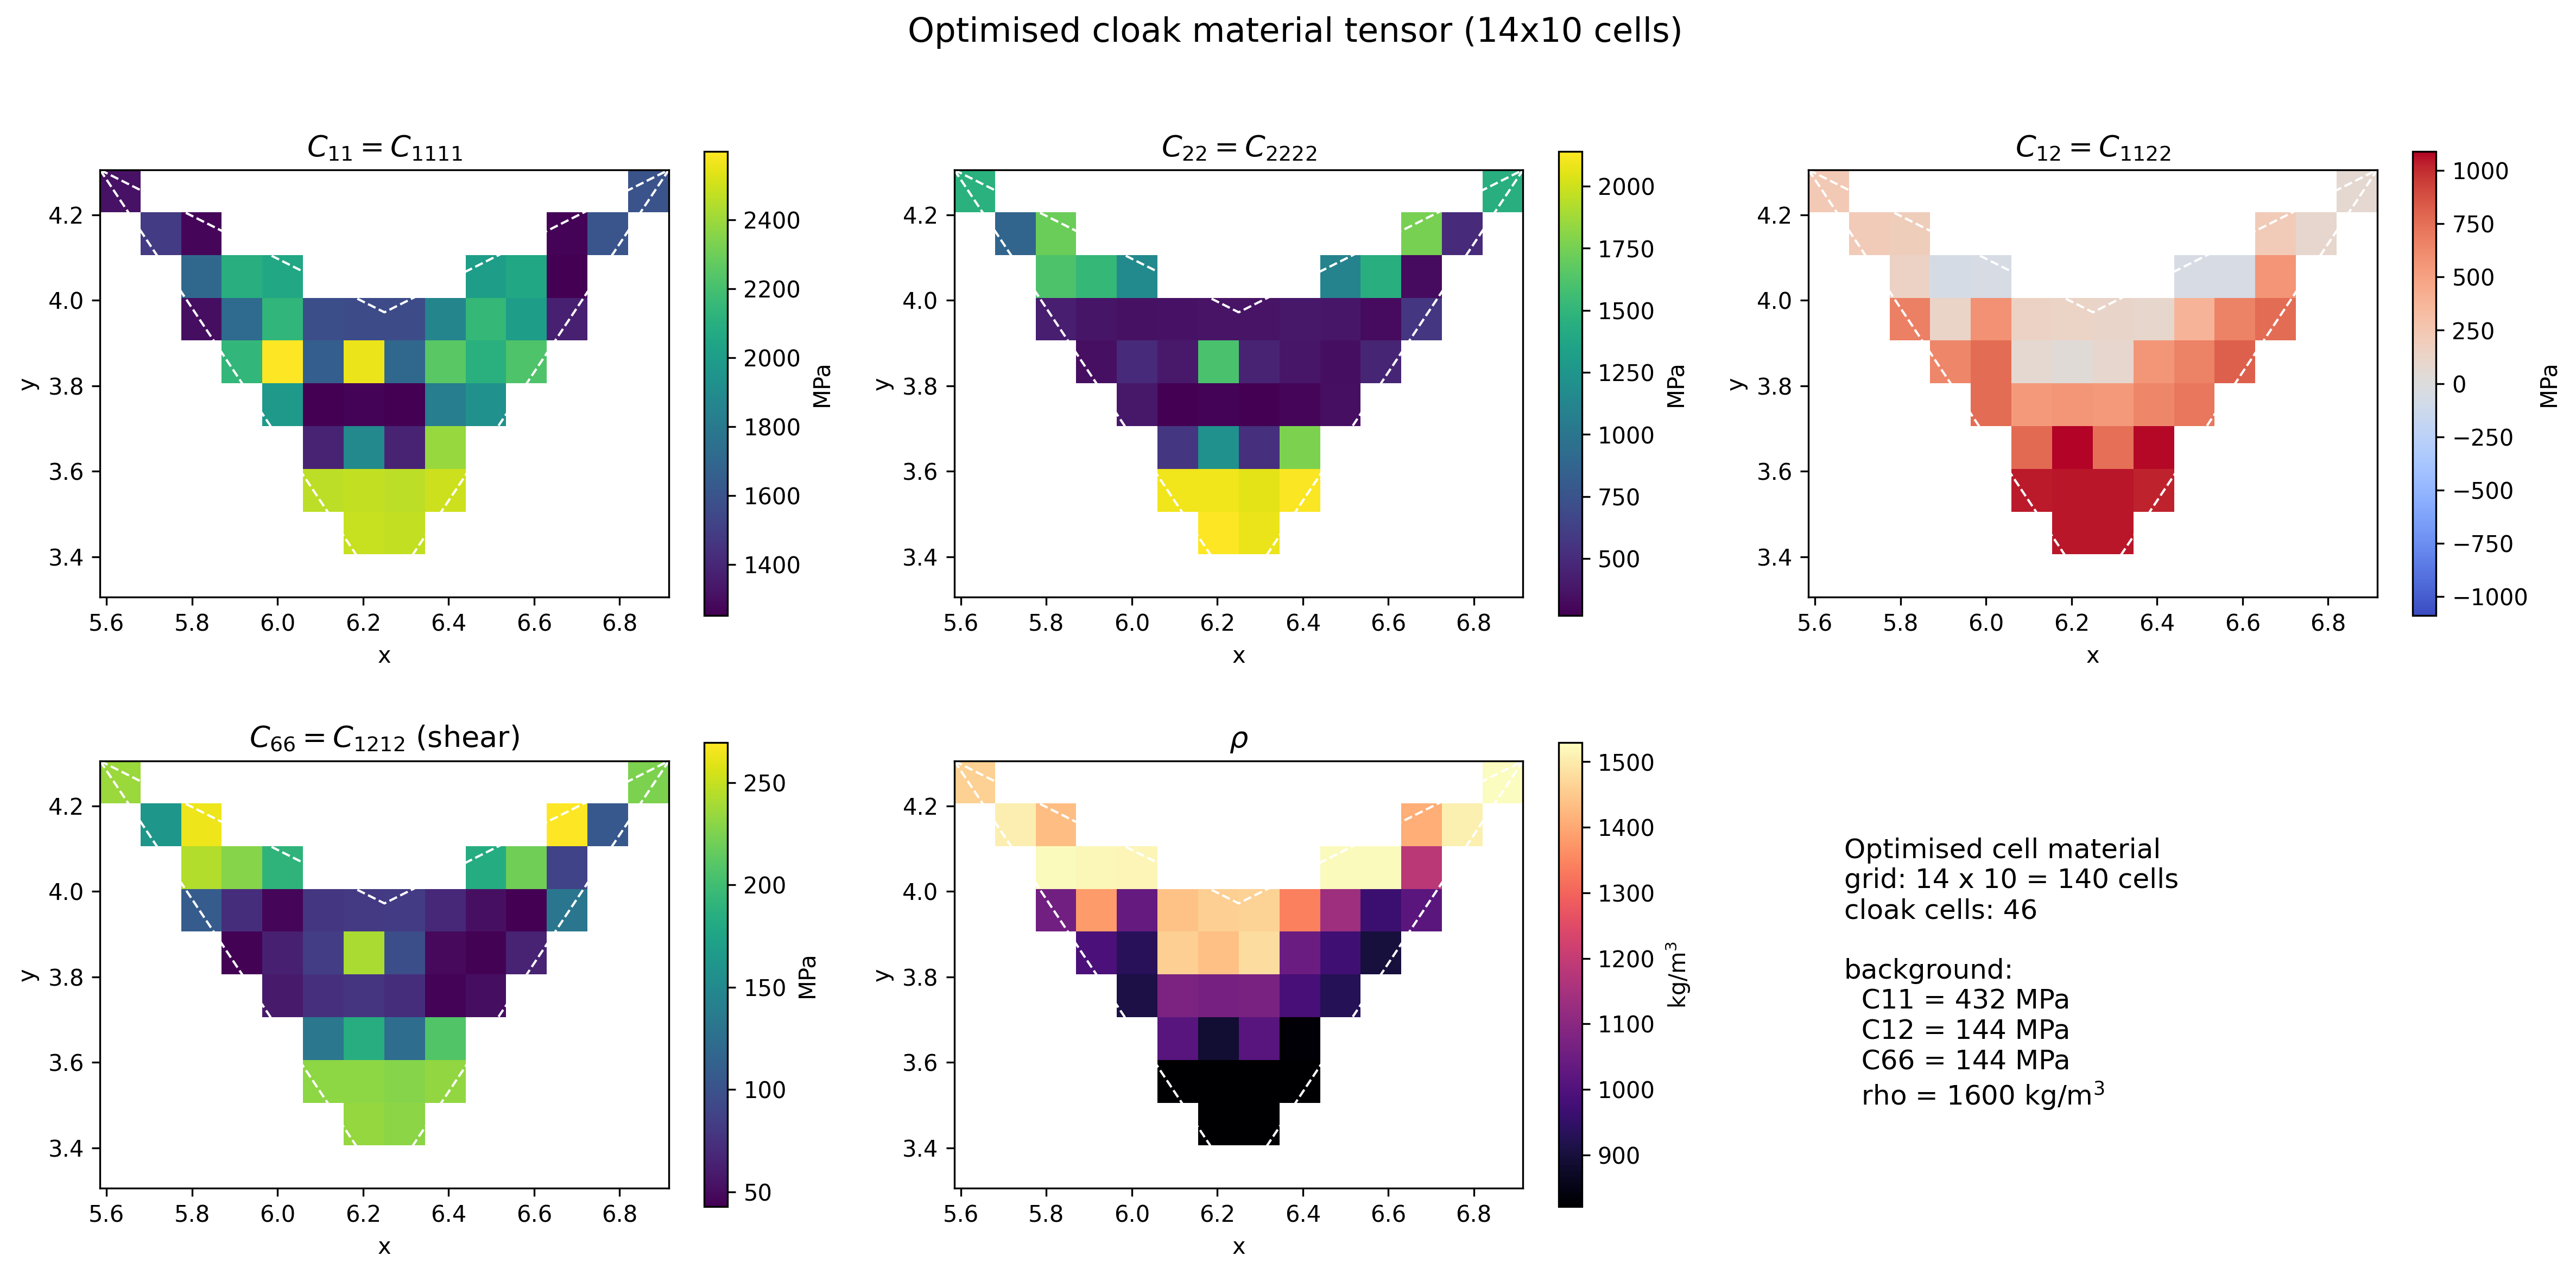
\includegraphics[width=\linewidth]{figures/single_freq_14x10_material.png}
  \caption{Optimised per-cell material of the $14\times10$ single-frequency
  cloak: the four orthotropic Cauchy moduli $C_{11},C_{22},C_{12},C_{66}$ and
  the density $\rho$ over the $46$ cells inside the cloak region (background
  cells masked). Only these $46$ materials are optimised.}
  \label{fig:single14_material}
\end{figure}

%% =============================================================
\section{Broadband multifrequency optimisation}\label{sec:multifreq}
%% =============================================================

\subsection{Single-frequency overfitting}

A neural-field cloak trained at a single design frequency $f^\star$
overfits aggressively: the cloak loss exhibits a sharp minimum at
$f^\star$ and degrades quickly away from it
(Fig.~\ref{fig:freq_overfitting}). Two independent runs trained at
$f^\star=2.5$ and $f^\star=3.0$ produce cloaks whose responses are
nearly disjoint outside a band of width $\Delta f^\star\approx0.2$
around their respective design frequencies. This behaviour is structurally identical to
narrow-band overfitting in topology-optimised acoustic cloaks
\citep{andkjaer2013} and motivates a multifrequency training objective.

\begin{figure}[htbp]
  \centering
  
\includegraphics[width=0.85\linewidth]{single_freq_comparison.png}
  \caption{Frequency response of two independently optimised
  $50\times50$ % TODO confirm grid (14×10?)
  neural-field cloaks, each trained at a single frequency
  ($f^\star=2.5$ and $f^\star=3.0$). The sharp minima at the
  training frequencies illustrate frequency-specific overfitting.}
  \label{fig:freq_overfitting}
\end{figure}

\subsection{Reference sweeps}\label{subsec:ref_sweeps}

Before introducing the optimised broadband design we record two
reference frequency sweeps on the chosen $50\times50$ % TODO confirm grid (14×10?)
cell decomposition: the ideal continuous $\mbf{c}_{\mathrm{eff}}$ cloak and
the uncoated defect (``obstacle''). Both are evaluated on the same
$N$-point grid $\{f_1,\dots,f_N\}$ spanning the target band
$[f_{\min},f_{\max}]$. The ideal sweep furnishes the lower envelope
attainable without microstructure constraints; the obstacle sweep is
the worst-case upper envelope. Together they bound the optimisation
target and let us state per-frequency cloaking quality as a fraction of
the available gap (Sec.~\ref{subsec:ratio_chart}).
Figure~\ref{fig:reference_sweeps} reports both.

\begin{figure}[htbp]
  \centering
  \includegraphics[width=0.8\linewidth]{reference_sweeps.png}
  \caption{Reference frequency sweeps on the target band: continuous
  $\mbf{c}_{\mathrm{eff}}$ cloak (lower envelope) and uncoated defect
  (upper envelope). Shaded region is the gap closed by optimisation.}
  \label{fig:reference_sweeps}
\end{figure}

\subsection{Min--max/mean objective}

For a target frequency band $\{f_1,\dots,f_N\}$ we replace
$\mcl{L}_{\mathrm{cloak}}$ in~\eqref{eq:opt_loss} by the convex
combination
\be\label{eq:minmax}
  \mcl{L}_{\mathrm{band}}(\theta)
  = \alpha\,\max_i \mcl{L}(f_i;\theta)
  + (1-\alpha)\,\frac{1}{N}\sum_i \mcl{L}(f_i;\theta),
\ee
with $\alpha$ annealed from $1$ to $0$ during training. The pure
min--max regime ($\alpha=1$) prevents the optimiser from trading
performance at one frequency for another; relaxing $\alpha$ towards $0$
sharpens the final solution once the loss landscape has been levelled.
Figure~\ref{fig:multifreq_sweep} shows that this schedule produces a
flat, low loss over the entire target band $f^\star\in[1.0,\,4.0]$.

\begin{figure}[htbp]
  \centering
  
\includegraphics[width=0.7\linewidth]{multifreq_sweep.png}
  \caption{Frequency sweep of a single $50\times50$ % TODO confirm grid (14×10?)
  neural-field cloak optimised with the multifrequency
  objective~\eqref{eq:minmax}.}
  \label{fig:multifreq_sweep}
\end{figure}

\subsection{Cloaking ratio across the band}\label{subsec:ratio_chart}

The dimensionless cloak ratio
$\eta(f) = \langle|\mbf{u}_{\mathrm{cloak}}(f)|\rangle / \langle|\mbf{u}_{\mathrm{ref}}(f)|\rangle$
on the free surface beyond the cloak is reported across the target band in
Figure~\ref{fig:u_ratio}. The optimised neural-field cloak holds
$\eta\approx 1$ throughout the band; the obstacle remains far from
unity and the ideal cloak provides a moving target close to but not
identically one (the residual gap is the mesh-convergence floor of
Sec.~\ref{subsec:mesh_conv}). The same ratio is the objective used in
the microstructure-constrained pipeline of Sec.~\ref{sec:micro}.

\begin{figure}[htbp]
  \centering
  \includegraphics[width=0.8\linewidth]{u_ratio_chart.png}
  \caption{Cloaking ratio
  $\eta(f)=\langle|\mbf{u}|\rangle/\langle|\mbf{u}_{\mathrm{ref}}|\rangle$
  on the free surface beyond the cloak across the target band, for the
  obstacle, the continuous $\mbf{c}_{\mathrm{eff}}$ cloak, and the
  optimised neural-field cloak. A flat $\eta\approx 1$ is the broadband
  cloaking ideal.}
  \label{fig:u_ratio}
\end{figure}

\subsection{Floquet--Bloch dispersion}\label{subsec:bloch}

To verify that the optimised broadband material is physically
admissible we compute the Floquet--Bloch dispersion of a vertical
strip unit cell cut through the optimised cloak, Bloch-periodic along
the surface direction $x_1$, traction-free at the top and fixed at the
bottom, following the construction used for the Rayleigh-wave
benchmark~\citep{chatzopoulos2023}. Because the triangular
transformation is invariant along $x_1$, the cell width is
unconstrained. Figure~\ref{fig:bloch} reports the lowest surface
branches over the reduced Brillouin zone $k_{x_1}\in(0,\pi/L_c]$.
The dispersion is real-valued across the target band — the optimised
cell supports propagating surface modes and does not rely on locally
resonant bandgaps to suppress transmission-side amplitude.
\begin{figure}[htbp]
  \centering
  \includegraphics[width=0.7\linewidth]{bloch_dispersion.png}
  \caption{Floquet--Bloch dispersion of a vertical strip unit cell
  through the broadband neural-field cloak, Bloch-periodic along the
  surface direction. Shaded band is the broadband training target.}
  \label{fig:bloch}
\end{figure}

\subsection{Results}

Figure~\ref{fig:sweep-compare} reports the per-frequency cloak loss of
the neural-field reparameterisation across the target band.
The neural-field run produces a flat, low response across the entire band,
reaching a band-averaged metric value of $0.985$. % confirm 4CM
Figure~\ref{fig:mat-compare} shows the optimised $(C,\rho)$ fields; the
neural field, unconstrained by a prior and fed high-order Fourier
features, produces sharp designs with fine spatial features.
Floquet--Bloch analysis of the multifrequency optimum
(Sec.~\ref{subsec:bloch}) confirms that the resulting unit cell supports
the propagation regime expected at the band centre.

\begin{figure}[htbp]
  \centering
  
\includegraphics[width=0.7\linewidth]{frequency_sweep_vis_NF.png}
  \caption{Per-frequency cloak loss of the neural-field reparameterisation
  across the target band. The broadband training flattens the response
  with respect to single-frequency optimisation.}
  \label{fig:sweep-compare}
\end{figure}

\begin{figure}[htbp]
  \centering
  \includegraphics[width=\linewidth,height=0.38\textheight,keepaspectratio]{material_field_NF.png}
  \caption{Optimised $(C,\rho)$ material fields produced by the
  neural-field reparameterisation.}
  \label{fig:mat-compare}
\end{figure}

%% =============================================================
\section{Microstructure-constrained optimisation}\label{sec:micro}
%% =============================================================

The cloaks of Sec.~\ref{sec:multifreq} are tensor-valued: each cell
carries a homogenised $(C,\rho)$ that need not correspond to any
realisable microstructure. We now constrain the neural field to a
manifold of physically realisable two-phase microstructures, following
the dataset-generation strategy of \citet{yang2024} for density-based
mechanical metamaterials.

\subsection{Dataset and homogenisation}

A dataset of $N\sim 10^{6}$ binary $50\times50$ unit cells is
generated by a squared-assembly cellular automaton on a
cement/void substrate. Periodic-FEM homogenisation on each unique cell
yields effective Lam\'e parameters
$(\lambda_{\mathrm{eff}},\mu_{\mathrm{eff}})$, density
$\rho_{\mathrm{eff}}$, and the full effective stiffness tensor
$C_{\mathrm{eff}}$. The construction follows~\citet{yang2024} in
shape and generative philosophy (binary CA + homogenisation) but is
specialised to the elastodynamic cloak target rather than to static
stiffness/Poisson design.

\subsection{Dataset distribution}\label{subsec:dataset_dist}

Figure~\ref{fig:dataset_dist} shows the marginal and pairwise
distributions of the homogenised descriptors
$(\lambda_{\mathrm{eff}},\mu_{\mathrm{eff}},\rho_{\mathrm{eff}})$ over
the $N\sim 10^6$ cell catalogue, with the trajectory traced by the
single-frequency optimum overlaid. The dataset covers a band-limited
region of the $(\lambda,\mu,\rho)$ space; the cloak-relevant portion
of the analytical $\mbf{c}_{\mathrm{eff}}$ map -- shown as the dashed
locus -- partially exits the dataset envelope, anticipating
the projection error quantified in Sec.~\ref{subsec:micro_results}.

\begin{figure}[htbp]
  \centering
  \includegraphics[width=0.95\linewidth]{dataset_distribution.png}
  \caption{Joint distribution of homogenised
  $(\lambda_{\mathrm{eff}},\mu_{\mathrm{eff}},\rho_{\mathrm{eff}})$ over
  the cellular-automaton dataset. Dashed locus: analytical
  $\mbf{c}_{\mathrm{eff}}$ map across the cloak. Coloured
  points: per-cell optimum of the constrained single-frequency design
  before snap-to-dataset.}
  \label{fig:dataset_dist}
\end{figure}

\subsection{GMM prior and constrained loss}

A Gaussian mixture is fit to the standardised
$(\lambda_{\mathrm{eff}},\mu_{\mathrm{eff}},\rho_{\mathrm{eff}})$ point
cloud, and a flat-top threshold $\tau$ at the $q$-th log-density
quantile defines the realisable manifold $\mcl{M}$. Since the cellular-automaton dataset is intrinsically Cauchy, the neural
field here uses the 4CM parameterisation (four free orthotropic Cauchy
moduli; Sec.~\ref{subsec:flat4}), summarised by the per-cell isotropic
descriptor $(\lambda_c,\mu_c,\rho_c)$. These parameters are optimised
through the neural field to
minimise the cloak loss together with a manifold-penalty
\be\label{eq:gmm_pen}
  \mcl{L}_{\mathrm{GMM}}
  = \sum_c \max\bigl(0,\,\tau - \log p_{\mathrm{GMM}}(\lambda_c,\mu_c,\rho_c)\bigr),
\ee
which pulls every cell into $\mcl{M}$ without forcing it onto a
specific dataset entry. After optimisation each cloak cell is snapped
to the dataset entry whose standardised
$(\lambda,\mu,\rho)$ is closest in Euclidean distance, and the resulting
matched microstructures tile the cloak region for pixel-level
validation on a refined mesh ($\sim$1 element per micro-pixel side).
Figure~\ref{fig:micro_pipeline} summarises the steps.

\begin{figure}[htbp]
  \centering
  \includegraphics[width=\linewidth]{pipeline.png}
  \caption{Microstructure-constrained pipeline: CA dataset generation
  $\to$ FEM homogenisation $\to$ GMM prior on
  $(\lambda,\mu,\rho)$ $\to$ neural-field optimisation with manifold
  penalty $\to$ snap-to-dataset $\to$ pixel-level FEM validation.}
  \label{fig:micro_pipeline}
\end{figure}

\subsection{Diagnostic experiment}\label{subsec:micro_results}

To separate the \emph{matching error} (projecting onto the discrete
dataset) from the \emph{pixel-vs.-homogenised error}, we add an
intermediate stage: each cloak cell's optimised
$(\lambda,\mu,\rho)$ is replaced by its matched dataset
$(\lambda,\mu,\rho)$, but the FEM is still run with a single
homogenised $(C,\rho)$ per cell rather than the actual pixel
microstructure. Table~\ref{tab:micro_results} reports the cloak ratio
$\langle|u|\rangle/\langle|u_{\mathrm{ref}}|\rangle$ at
$f^\star=2.0$ on a $20\times15$ macro grid with $100$
cloak cells.

\begin{table}[htbp]
\centering
\caption{Microstructure-constrained results: cloak ratio at
$f^{\star}=2.0$. Mesh refinement does not close the
matched-vs-validated gap.}
\label{tab:micro_results}
\begin{tabular*}{\textwidth}{@{}lll@{}}
\toprule
Configuration & $\langle|u|\rangle/\langle|u_{\mathrm{ref}}|\rangle$ & mesh refinement \\
\midrule
Optimised (homogenised, free $\lambda,\mu,\rho$)       & $\approx 1.00$ & 3  \\
Matched (homogenised, dataset $\lambda,\mu,\rho$)      & $0.9385$       & 3  \\
Matched (homogenised, dataset $\lambda,\mu,\rho$)      & $0.9544$       & 20 \\
Validated (pixel-level, real microstructure)           & $\approx 0.70$ & 25 \\
\bottomrule
\end{tabular*}
\end{table}

\paragraph{The $\sim$5\% matching gap is benign.}
Going from the free optimum ($1.00$) to the matched homogenised cloak
($0.94$--$0.95$) costs about five percentage points. This is the price
of projecting onto a discrete dataset and is straightforwardly improved
by (i)~enlarging the dataset, (ii)~reweighting the matching distance so
that $\mu$ is not effectively ignored, or (iii)~replacing nearest-neighbour
snap with a generative match.

\paragraph{The $\sim$25\% pixel-vs-homogenised gap is the real problem.}
Once the matched entries are inserted as actual microstructures the
cloak ratio collapses to $\sim$0.70 and mesh refinement does not close
the gap. The most likely cause is hidden anisotropy: the descriptor
$(\lambda,\mu)$ is an isotropic projection of an effective stiffness
that is generally orthotropic, and two microstructures with the same
$(\lambda,\mu)$ but different principal axes scatter waves very
differently. Dynamic-homogenisation effects (Willis
couplings~\citep{willis1981}) and pixel-level scattering at
cement/void interfaces are secondary candidate causes. A disambiguating
experiment in which the full anisotropic $C$ tensor of each matched
microstructure is recomputed and reinserted will determine whether the
gap is removable in principle by storing and optimising over anisotropic
moduli, or whether it is a genuinely finite-wavelength effect that
requires either dynamic homogenisation or direct optimisation in
microstructure space.

\subsection{Displacement-field validation}\label{subsec:disp_validation}

Figure~\ref{fig:disp_validation} compares the displacement field of the
matched homogenised cloak with the pixel-level validation on the
refined mesh. The transmission-side amplitude is well reconstructed by the
homogenised solve but the pixel-level field carries higher-order
features near cell interfaces that the descriptor
$(\lambda,\mu,\rho)$ cannot encode. These features are the visual
correlate of the $\sim$25\% pixel-vs-homogenised gap quantified in
Table~\ref{tab:micro_results}.

\begin{figure}[htbp]
  \centering
  \includegraphics[width=\linewidth]{displacement_field_validation.png}
  \caption{Displacement-field validation at $f^\star=2.0$. Left:
  reference (defect-free). Centre: matched homogenised cloak. Right:
  pixel-level validation on the refined mesh. Insets zoom into the
  cloak interior to highlight scattering at cement/void interfaces.}
  \label{fig:disp_validation}
\end{figure}

\subsection{Microstructure gallery}\label{subsec:micro_gallery}

Figure~\ref{fig:micro_gallery} shows a representative sample of the
matched cement/void microstructures tiled across the cloak. Each
panel is a $50\times50$ binary unit cell from the snap-to-dataset
matching of Sec.~\ref{subsec:micro_results}; the colour outline encodes
the position of the host cell in the cloak, illustrating
the gradient from strongly sheared, low-density configurations near the
defect boundary to near-bulk configurations at the outer boundary.

\begin{figure}[htbp]
  \centering
  \includegraphics[width=\linewidth]{microstructure_gallery.png}
  \caption{Gallery of matched cement/void microstructures tiling the
  cloak. Each panel is a $50\times50$ binary unit cell from the dataset;
  outline colour encodes the position of the host macro cell in the cloak.}
  \label{fig:micro_gallery}
\end{figure}

%% =============================================================
\section{Broadband microstructure-constrained design}\label{sec:micro_band}
%% =============================================================

The single-frequency microstructure pipeline of Sec.~\ref{sec:micro}
extends to the broadband regime by combining the GMM manifold penalty
of Eq.~\eqref{eq:gmm_pen} with the multifrequency
objective~\eqref{eq:minmax}. We retain the 4CM stiffness
parameterisation of Sec.~\ref{subsec:flat4} -- the cellular-automaton
dataset is intrinsically Cauchy and is fully covered by the four
orthotropic Cauchy moduli -- and train a single neural field against
\be\label{eq:micro_band_loss}
  \mcl{L}_{\mathrm{band+micro}}(\theta)
  = \mcl{L}_{\mathrm{band}}(\theta)
  + \lambda_{\mathrm{GMM}}\,\mcl{L}_{\mathrm{GMM}}(\theta)
  + \lambda_{\ell_2}\,\mcl{L}_{\ell_2}(\theta).
\ee
The manifold penalty is annealed from a small initial value so that
the broadband cloak loss can shape the geometry before the GMM
constraint tightens around the realisable region.

\paragraph{Snap, validate, sweep.} After optimisation we snap the
per-cell parameters to the nearest dataset entry (as in
Sec.~\ref{sec:micro}) and run a frequency sweep on the matched
homogenised cloak across the same band used in Sec.~\ref{sec:multifreq}.
Figure~\ref{fig:micro_band_sweep} reports the cloaking ratio
$\eta(f)$ across the band, alongside the reference and obstacle sweeps
of Sec.~\ref{subsec:ref_sweeps}. The broadband micro-constrained cloak
retains a roughly flat profile -- evidence that the GMM penalty does
not collapse the design to a single-frequency optimum -- but exhibits
the same residual amplitude penalty isolated in
Sec.~\ref{subsec:micro_results}.

\begin{figure}[htbp]
  \centering
  \includegraphics[width=0.8\linewidth]{multifreq_micro_sweep.png}
  \caption{Frequency sweep of the broadband
  microstructure-constrained cloak: cloaking ratio
  $\eta(f)=\langle|\mbf{u}|\rangle/\langle|\mbf{u}_{\mathrm{ref}}|\rangle$
  for the matched homogenised cloak (solid) and the pixel-level
  validation on the refined mesh (dashed), against the reference
  envelopes.}
  \label{fig:micro_band_sweep}
\end{figure}

%% =============================================================
\section{Discussion}\label{sec:discussion}
%% =============================================================

The three regimes above share a single architectural choice -- a
coordinate-conditioned neural field on top of a differentiable FEM --
and they show, in different forms, the same advantage over hand-crafted
symmetrisation strategies. In the single-frequency case the network finds a low-distortion realisable
cloak by directly searching four orthotropic Cauchy moduli per cell; the
broken minor symmetry belongs to the ideal polar tensor and represents the
gap that any realisable Cauchy design (ours included) must approximate. In
the multifrequency case the network's implicit smoothness eliminates
the spurious cell-to-cell oscillations that plague raw per-cell
optimisation and the band objective flattens the loss across a wide
target band. In the microstructure-constrained case the same network
output is projected onto a realisability manifold, and the resulting
diagnostic isolates a homogenisation gap that is hidden in pure
tensor-level designs.

\paragraph{Comparison with prior work.} \citet{wang2022} use the same
type of $L^2$ outside-cloak metric in an elasto-static setting and
report a reduction from $17.2\%$ in the voided structure to $4\%$ in
the cloaked structure for a circular-void cloak with a database of
orthotropic unit cells. Under the analogous metric our continuous
$\mbf{c}_{\mathrm{eff}}$ cloak reduces the outside distortion from
$\sim\!5\%$ to an extrapolated $\sim\!0.75\%$, and the optimised
$14\times10$ neural-field cloak attains $\sim\!1.7\%$. % confirm 4CM
The comparison is not strictly apples-to-apples -- our setting is
frequency-domain elastodynamic (the ideal cloak is polar; our realisable
design is orthotropic Cauchy 4CM), theirs is quasi-static and Cauchy -- but the order of magnitude is encouraging. The
microstructure-constrained results sit between the two regimes and
make explicit the (sub)gap that any pure tensor-level optimisation has
been silently hiding.

\paragraph{Limitations.} The cell discretisation imposes a piecewise-constant
material approximation whose square cells cannot conform exactly to the
inclined cloak interfaces; the residual right-boundary distortion of the
continuous tensor is dominated by FEM error rather than by an intrinsic
limit of the transformation. The microstructure pipeline is currently
restricted to a two-phase binary substrate and to an isotropic
$(\lambda,\mu,\rho)$ descriptor; the anisotropic generalisation
proposed in Sec.~\ref{sec:micro} is the natural next step.

\paragraph{Future work.} The most direct extension is to stop snapping
to a discrete database altogether and to learn a generative model of
the realisable manifold that can be queried differentiably during
optimisation (e.g.\ a guided diffusion model in the spirit
of~\citet{yang2024}). A second extension is to incorporate dynamic
homogenisation or Willis-type effective tensors into the
microstructure descriptor, which we expect to close most of the
remaining homogenisation gap. A third extension is to move from the
two-dimensional carpet cloak to three-dimensional configurations, for
which the differentiable JAX-FEM pipeline carries over without
qualitative change. A fourth extension is to design beyond the
four-parameter orthotropic Cauchy class by realising the broken minor
symmetry of the ideal polar tensor via Cosserat or polar microstructures,
directly closing the gap between the BGM prescription and the realisable
design.

%% =============================================================
\section{Conclusion}\label{sec:conclusion}
%% =============================================================

We have presented a unified, differentiable design pipeline for
two-dimensional Rayleigh-wave carpet cloaks in which the per-cell
material is parameterised by four free orthotropic Cauchy moduli
$(C_{11},C_{12},C_{22},C_{66})$ and a scalar density, searched by a
coordinate-conditioned neural field through an end-to-end differentiable
JAX-FEM pipeline. This is an alternative to closed-form arithmetic-mean
symmetrisation of the ideal polar tensor that directly explores the
realisable Cauchy design space; the ideal BGM transformation tensor (polar,
ten components) is retained as the mathematical reference, while all
optimised designs are Cauchy. The pipeline recovers near-perfect
single-frequency cloaking, flattens the cloak loss across a target
frequency band when trained with a min--max/mean objective, and can be
projected onto a realisability manifold of homogenised binary
microstructures to expose a hidden-anisotropy gap that has not, to our
knowledge, been isolated before in the elastodynamic regime.

%% Bibliography
\bibliographystyle{elsarticle-num-names}
\bibliography{cas-refs}

\end{document}
